% Masterthesis 
% Rico Leuthold 2.9.2008
%
%noTeXShop

%---------------------------------------------------------------------------------------------------------
% Document setup
%---------------------------------------------------------------------------------------------------------

% paper format and stylesheet
\documentclass[a4paper,10pt,twoside,headings=small,bibliography=totocnumbered,headsepline]{scrartcl}
%\usepackage[english,german,brazilian]{babel}

% praphic package
\usepackage{graphicx}

% titlepage
\usepackage{titlepic}

% Font
\usepackage{times}
\usepackage[T1]{fontenc} 
\usepackage[english]{babel}
\usepackage{color}

% orientation
\usepackage{rotating}
\usepackage{lscape}

% used for citations
\usepackage[square, numbers, super]{natbib}

% Links
\usepackage[pdftex,hyperfootnotes=false,pdfborder=0 0 0]{hyperref}
\definecolor{darkgrey}{rgb}{0.2,0.2,0.2}
\hypersetup{
    colorlinks,%
    citecolor=black,%
    filecolor=black,%
    linkcolor=darkgrey,%
    urlcolor=blue
}

\urlstyle{rm}

% tables
\usepackage{tabularx}
\usepackage{ctable}

% used for source code
\usepackage{listings}
\usepackage{fancyvrb}
\definecolor{lightgrey}{rgb}{0.95,0.95,0.95}

% appendix
\usepackage[toc,page]{appendix}

% heading on every page
\pagestyle{headings}

% Spacing
\frenchspacing

% ... some mor spacing stuff
\usepackage{setspace}


% border of pdf pics
\pdfpagebox 4

% Acronyms
\usepackage[printonlyused,withpage,footnote]{acronym}

%
% CUSTOM COMMANDS
%

% make inline listings normal font size
\makeatletter
\lst@AddToHook{TextStyle}{\let\lst@basicstyle\ttfamily\small\fontfamily{pcr}\selectfont}
\makeatother

% Code style with line numbers 
\newenvironment{numcodestyle}{
	\lstset{basicstyle=\footnotesize, numbers=left, numberstyle=\tiny, numbersep=3mm, stepnumber=1, backgroundcolor=\color{lightgrey}}
}

% Code style without line numbers
\newenvironment{codetiny}{
	\lstset{basicstyle=\tiny, numbers=none, backgroundcolor=\color{lightgrey}}
}

\newenvironment{codefoot}{
	\lstset{basicstyle=\footnotesize, numbers=none, backgroundcolor=\color{lightgrey}}
}

\newenvironment{codescript}{
	\lstset{basicstyle=\scriptsize, numbers=none, backgroundcolor=\color{lightgrey}}
}

% this makes description lists spacing much better.
\newenvironment{mydesc}{
	\begin{description}
	  \setlength{\itemsep}{1pt}
	  \setlength{\parskip}{0pt}
	  \setlength{\parsep}{0pt}
}
{
	\end{description}
}

% this makes list spacing much better.
\newenvironment{condensed_enum}{
	\begin{enumerate}
	  \setlength{\itemsep}{1pt}
	  \setlength{\parskip}{0pt}
	  \setlength{\parsep}{0pt}
}
{
	\end{enumerate}
}

% this makes list spacing much better.
\newenvironment{condensed_item}{
	\begin{itemize}
      \renewcommand{\labelitemi}{$\circ$}
	  \setlength{\itemsep}{1pt}
	  \setlength{\parskip}{0pt}
	  \setlength{\parsep}{0pt}
}
{
	\end{itemize}
}

% Table column types for bold row 
\newcolumntype{+}{>{\global\let\currentrowstyle\relax}}
\newcolumntype{^}{>{\currentrowstyle}}
\newcommand{\rowstyle}[1]{\gdef\currentrowstyle{#1}%
#1\ignorespaces
}

%===============================
% Start document
%===============================
\begin{document}

% select language
\selectlanguage{english}

% Title page
%\title{Informatic Tools to Explore Social Behavior in House Mice}
%\author{Rico Leuthold}
%\date{\today}  %\today is replaced with the current date
%\maketitle
\begin{titlepage}
\begin{flushleft}

\includegraphics[width=\textwidth]{assets/pdf/title_header.pdf}
\end{flushleft}
\vspace{2cm}
\begin{center}
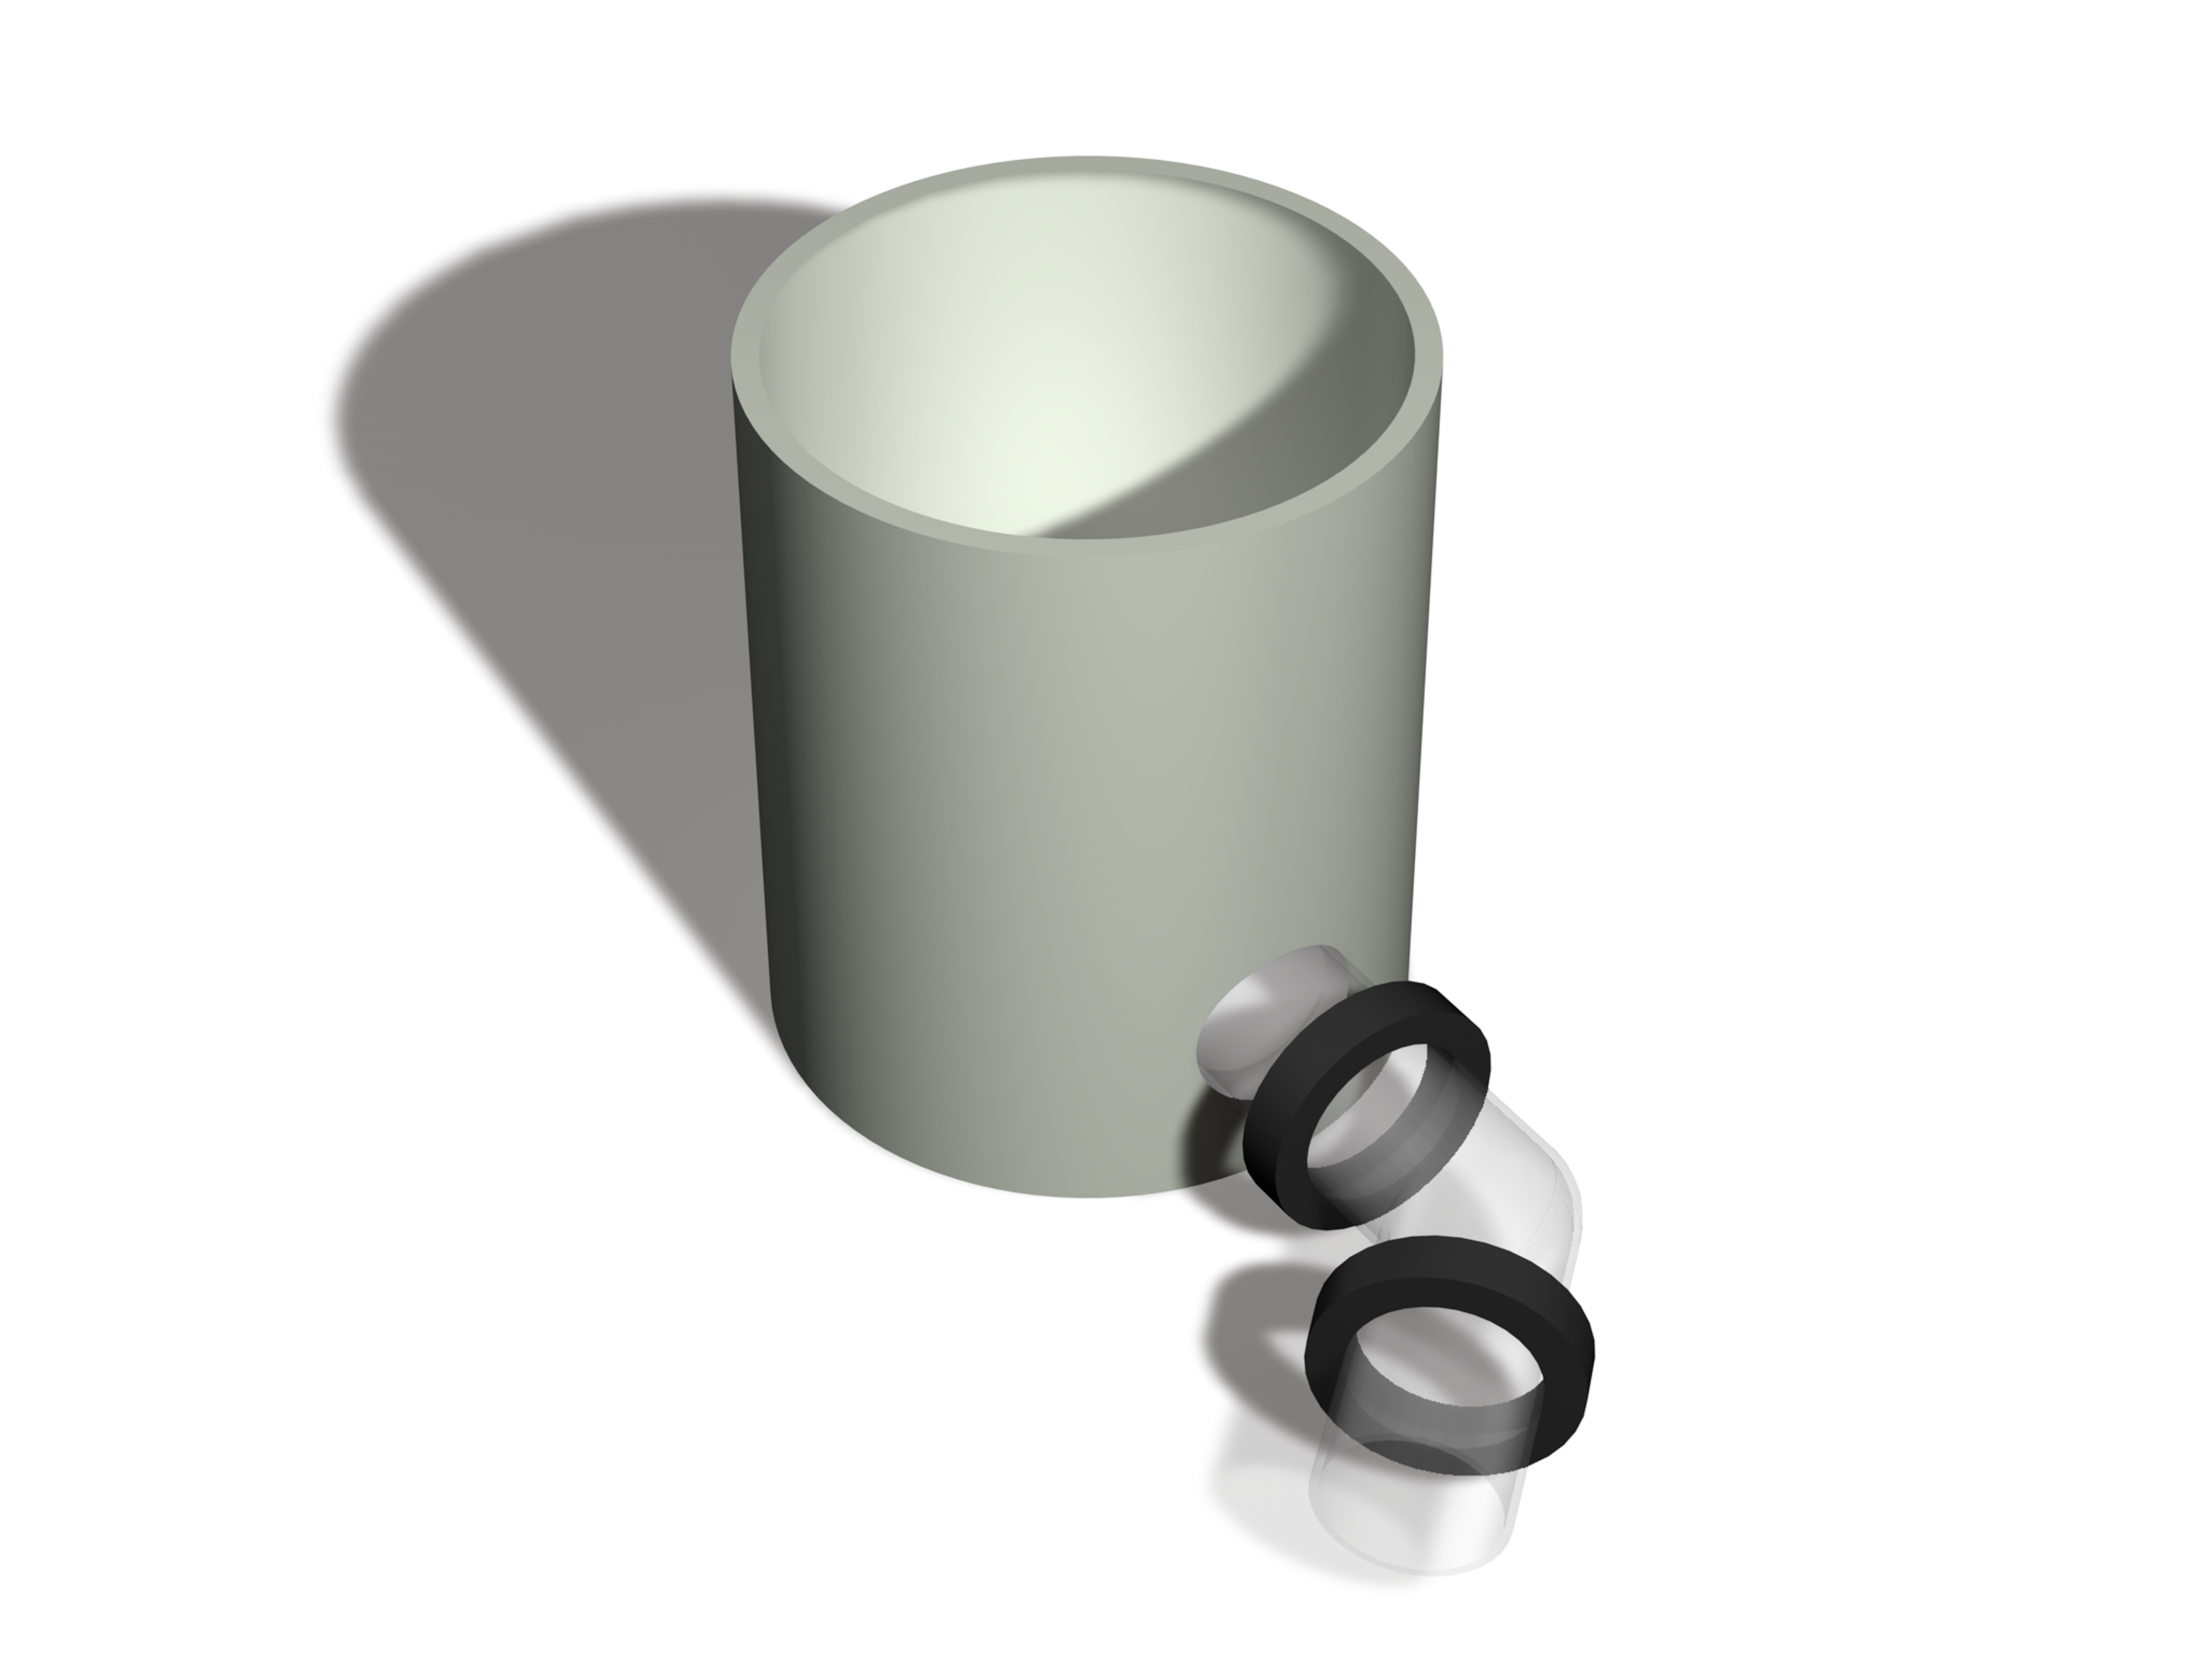
\includegraphics[width=\textwidth]{assets/pdf/box_title.pdf}
\end{center}


\vfill

% Author and supervisor
\begin{minipage}{0.5\textwidth}
	\begin{flushleft}
		
\includegraphics[width=\textwidth]{assets/pdf/title_footer_author.pdf}
	\end{flushleft}
\end{minipage}
\begin{minipage}{0.5\textwidth}
	\begin{flushright}
		
\includegraphics[width=\textwidth]{assets/pdf/title_footer_supervisor.pdf}
	\end{flushright}
\end{minipage}
\end{titlepage}

\newpage

% Table of contents
\tableofcontents
\listoftables
% add table of figures to toc
\listoffigures

% ===============================
% Introduction
% ===============================
% ===============================
% Introduction
% ===============================
\newpage

\section{Introduction}
\label{sec:introduction}

In May 2008, the research group around Prof. Barbara K\"onig at the Institute of Zoology of the University of Z\"urich decided to take their research in the field of animal behavior to the next level. Especially interested in the complex social behavior of house mice \textit{(Mus domesticus)} they came up with the idea to design an automated system to collect spatial position data of mice living in a barn.

\subsection{Motivation}
\label{subsec:motivation}
The motivation for such an effort is to obtain a statistically relevant set of data to develop, test and prove scientific hypothesis about the complex social behavior of house mice. An automated system has the advantage that it collects data 24 hours a day, and the mice are in no way disturbed in their natural behavior by the presence of an observer.

My personal motivation derives from the interest in informatics and my study in biology. The project gave me a lot of room to enhance my skills in informatics, while working on an interesting biological topic. Additionally, I am interested in the \textit{Social Network Analysis} to study complex social behavior.

The system collecting the data in the barn has been developed and constructed by a company called \textit{New Behaviour}, a company based in Z\"urich. Thus, the main objective of this work was to develop software to store data and make it accessible to researchers for analysis 

\subsection{Tasks}
\label{subsec:task}
Handling the spatial position data collected by the automated system is challenging, as it includes several tasks which can be carried out only using informatics on a level that biologists normally can not cope with.

\subsubsection{Storing and Accessing the Data}
\label{subsubsec:storeaccess}
The data collected by the automated system must be stored securely. Theredore, part of the approach is to set up a \ac{RDBMS} (RDBMS). 

Also, an intuitive user interface must be available, to access the data, facilitate data exploration, and export to other software applications. Furthermore, the technology used to create the interface should be cross-platform compatible, to ensure maximal accessibility.

\subsubsection{Additional Tasks}
\label{subsubsec:additional}
Additionally, the user should be provided with an interface to carry out some simple statistical analysis.

Last but not least, some functionality should enable to graphically display the social network, and export the data for a social network analysis. 

% ===============================
% Biology of the house mice
% ===============================
% ===============================
% Biology of the house mice
% ===============================
\newpage
\section{Biology of the house mouse}
\label{sec:biolhousemice}

\subsection{Introduction}
\label{subsec:introduction}

House mice (\textit{Mus domesticus}) (see Fig.~\ref{fig:housemice}) live under a multitude of different environmental conditions. The ecological success of house mice as a widely distributed species reflects the fact, that they are very flexible in terms of their social, territorial and reproductive behavior \citep{bronson:79, bronson:84, berry:81}. Under natural conditions house mice have a relatively low expectancy of life (100 to 150 days). During this short life span, female mice are avid to have as many offspring as possible. Living under optimal food conditions, a female mouse gives birth to a litter of 5-7 pups every four weeks \citep{berry:71, pelikan:81}. The juvenile mortality is estimated between 50\% and 85\% \citep{berry:71, berry:75, pennycuik:86}. Having heavier pups is an advantage, as they can be weaned faster, which positively influences future reproduction of the mother\citep{fuchs:82}. The litter size of a wild house mouse increases from the first to the second lactation and decreases after the fifth lactation \citep{pelikan:81, koenig:87b}. 

\begin{figure}[htbp]	
\centering	
\includegraphics[width=0.5\textwidth]{assets/pdf/mus_domesticus.pdf}	
\caption[House mouse]{House mouse \textit{(Mus domesticus).}}
\label{fig:housemice}
\end{figure}

\subsection{General social behavior}
\label{subsec:socialbehaviour}
House mice typically live in a social collective which forms a reproduction group. These groups usually include a dominant male, one or several females with their litters and possibly some subordinate males \citep{crowcroft:63, reimer:67, selander:70, mackintosh:81}.

The mating habit is typically polygynandric (both males and females have several mating partners), but monogamic living pairs have also been reported \citep{lidicker:76}. Juvenile females may stay in the territory of their parents to raise their own offspring \citep{petras:67}. There is evidence of stranger females immigrating into social groups as well \citep{anderson:65, reimer:67, selander:70, bronson:79, baker:81}.     

\subsection{Research topics}
\label{subsec:researchtopics}

The research group in animal behavior around Prof. K\"onig at the University of Z\"urich is generally interested in the complex social behavior of the house mice. Mainly the influence of the social partner choice, other then mating, onto the fitness of the female mice, is in the focus of the studies. Such social selection occurs, if social interactions result in favorable fitness consequences. Therefore, reproductive cooperation such as joint nesting, for example, should manifest in an increased number of offspring \citep{weidt:07}. Cooperative interactions can extend to sharing of brood-rearing duties like nursing.

\subsubsection{Communal nursing}
\label{subsubsec:comnurs}

Over forty years ago, first observations of wild female house mice, belonging to the same reproduction group, which raise their pups in communal nests have been reported \citep{southwick:55}. Ever since, this behavior has been noticed for house mice living under all kind of environmental conditions.\citep{crowcroft:63, sayler:69, gandelman:70, werboff:70, baker:81}.

This behavior is astonishing, as the energetic costs of lactation are very high, hence influence the females' future reproduction success. To wean a litter of about seven to eight pups, the mother has to produce 100 grams of milk within 22 days, which is equivalent to 1100 \acf{KJ} \citep{koenig:88}. Depending on the size of the litter and the duration of the lactation phase, the length of the interbirth intervals change \citep{fuchs:81, fuchs:82, koenig:87a, koenig:87b}.

Several experiments have been carried out with wild house mice living under laboratory conditions. Manipulating group size and the composition of the group in terms of relatedness of the individuals revealed that non-offspring nursing is an integral part of the reproductive behavior of female house mice in egalitarian groups. However, the probability for such mutualistic cooperation was highest when a female shared a nest with a familiar sister to form a low-skew society \citep{koenig:06}.

According to K\"onig \citep{koenig:06}, the direct benefits of allomaternal care for the pups could be diverse. As there are, improved survival, improved future reproduction, improved growth or immunological benefits.

There are physiological benefits for the mother as well, which lead to an increase of their reproductive output. Of notable interest is the hypothesis named \textit{Metabolic peak load reduction}. Explained in short, a solitary nursing female tends to have a peak of energy consumption during the nursing phase of her litter. Nevertheless, female house mice are limited in their maximal sustainable metabolism \citep{hammond:92}. This limit depends on the age and physique of the individual and is called \textit{metabolic ceiling}. Partial synchronization in reproduction within the females of a group, combined with the communal nursing, can balance the energy demand for the individual, as the burden of nursing the litter is divided. Hence, the energy demand for each female stays always on a medium level\citep{koenig:06}. This can result in an increased lifetime reproduction success.

However, due to the artificial setup of the experiments, no conclusion about the communal nursing under natural conditions could be made.


% ===============================
% Shed setup
% ===============================
% ===============================
% Shed setup
% ===============================
\newpage
\section{Experiment set-up}
\label{sec:shedsetup}

Since 2003 the K\"onig lab studies a wild population of house mice in a barn, where mice can leave and enter freely.

The barn is located in a forest near Illnau (Switzerland) and consist of a single room with an area of 64m$^2$ (12.8m x 5.75m). Stable plastic walls (height \textasciitilde50cm) divide the area into four segments and an entry space. Small transit holes in the dividers ensure access to the different segments (Fig.~\ref{fig:barn_schema}).

The entry area provides workspace for the researchers and is used to store tools and material. Furthermore, the central computer for the data collection system (see section \ref{subsec:collectspatialpos}) is placed in this area.

The 40 artificial nestboxes (see figure~\ref{fig:artNestbox} for a schematic model) are distributed evenly in the four sectors (see figure~\ref{fig:barn_schema} for the current positioning of the boxes) along with some plastic pipe structures, bricks, smaller plastic walls and shelters to structure the environment (Fig.~\ref{fig:shedoverview}). These structuring elements ensure the existence of several territories, and provide hideouts for the subordinate mice.

\begin{figure}[htpb]
\begin{center}
  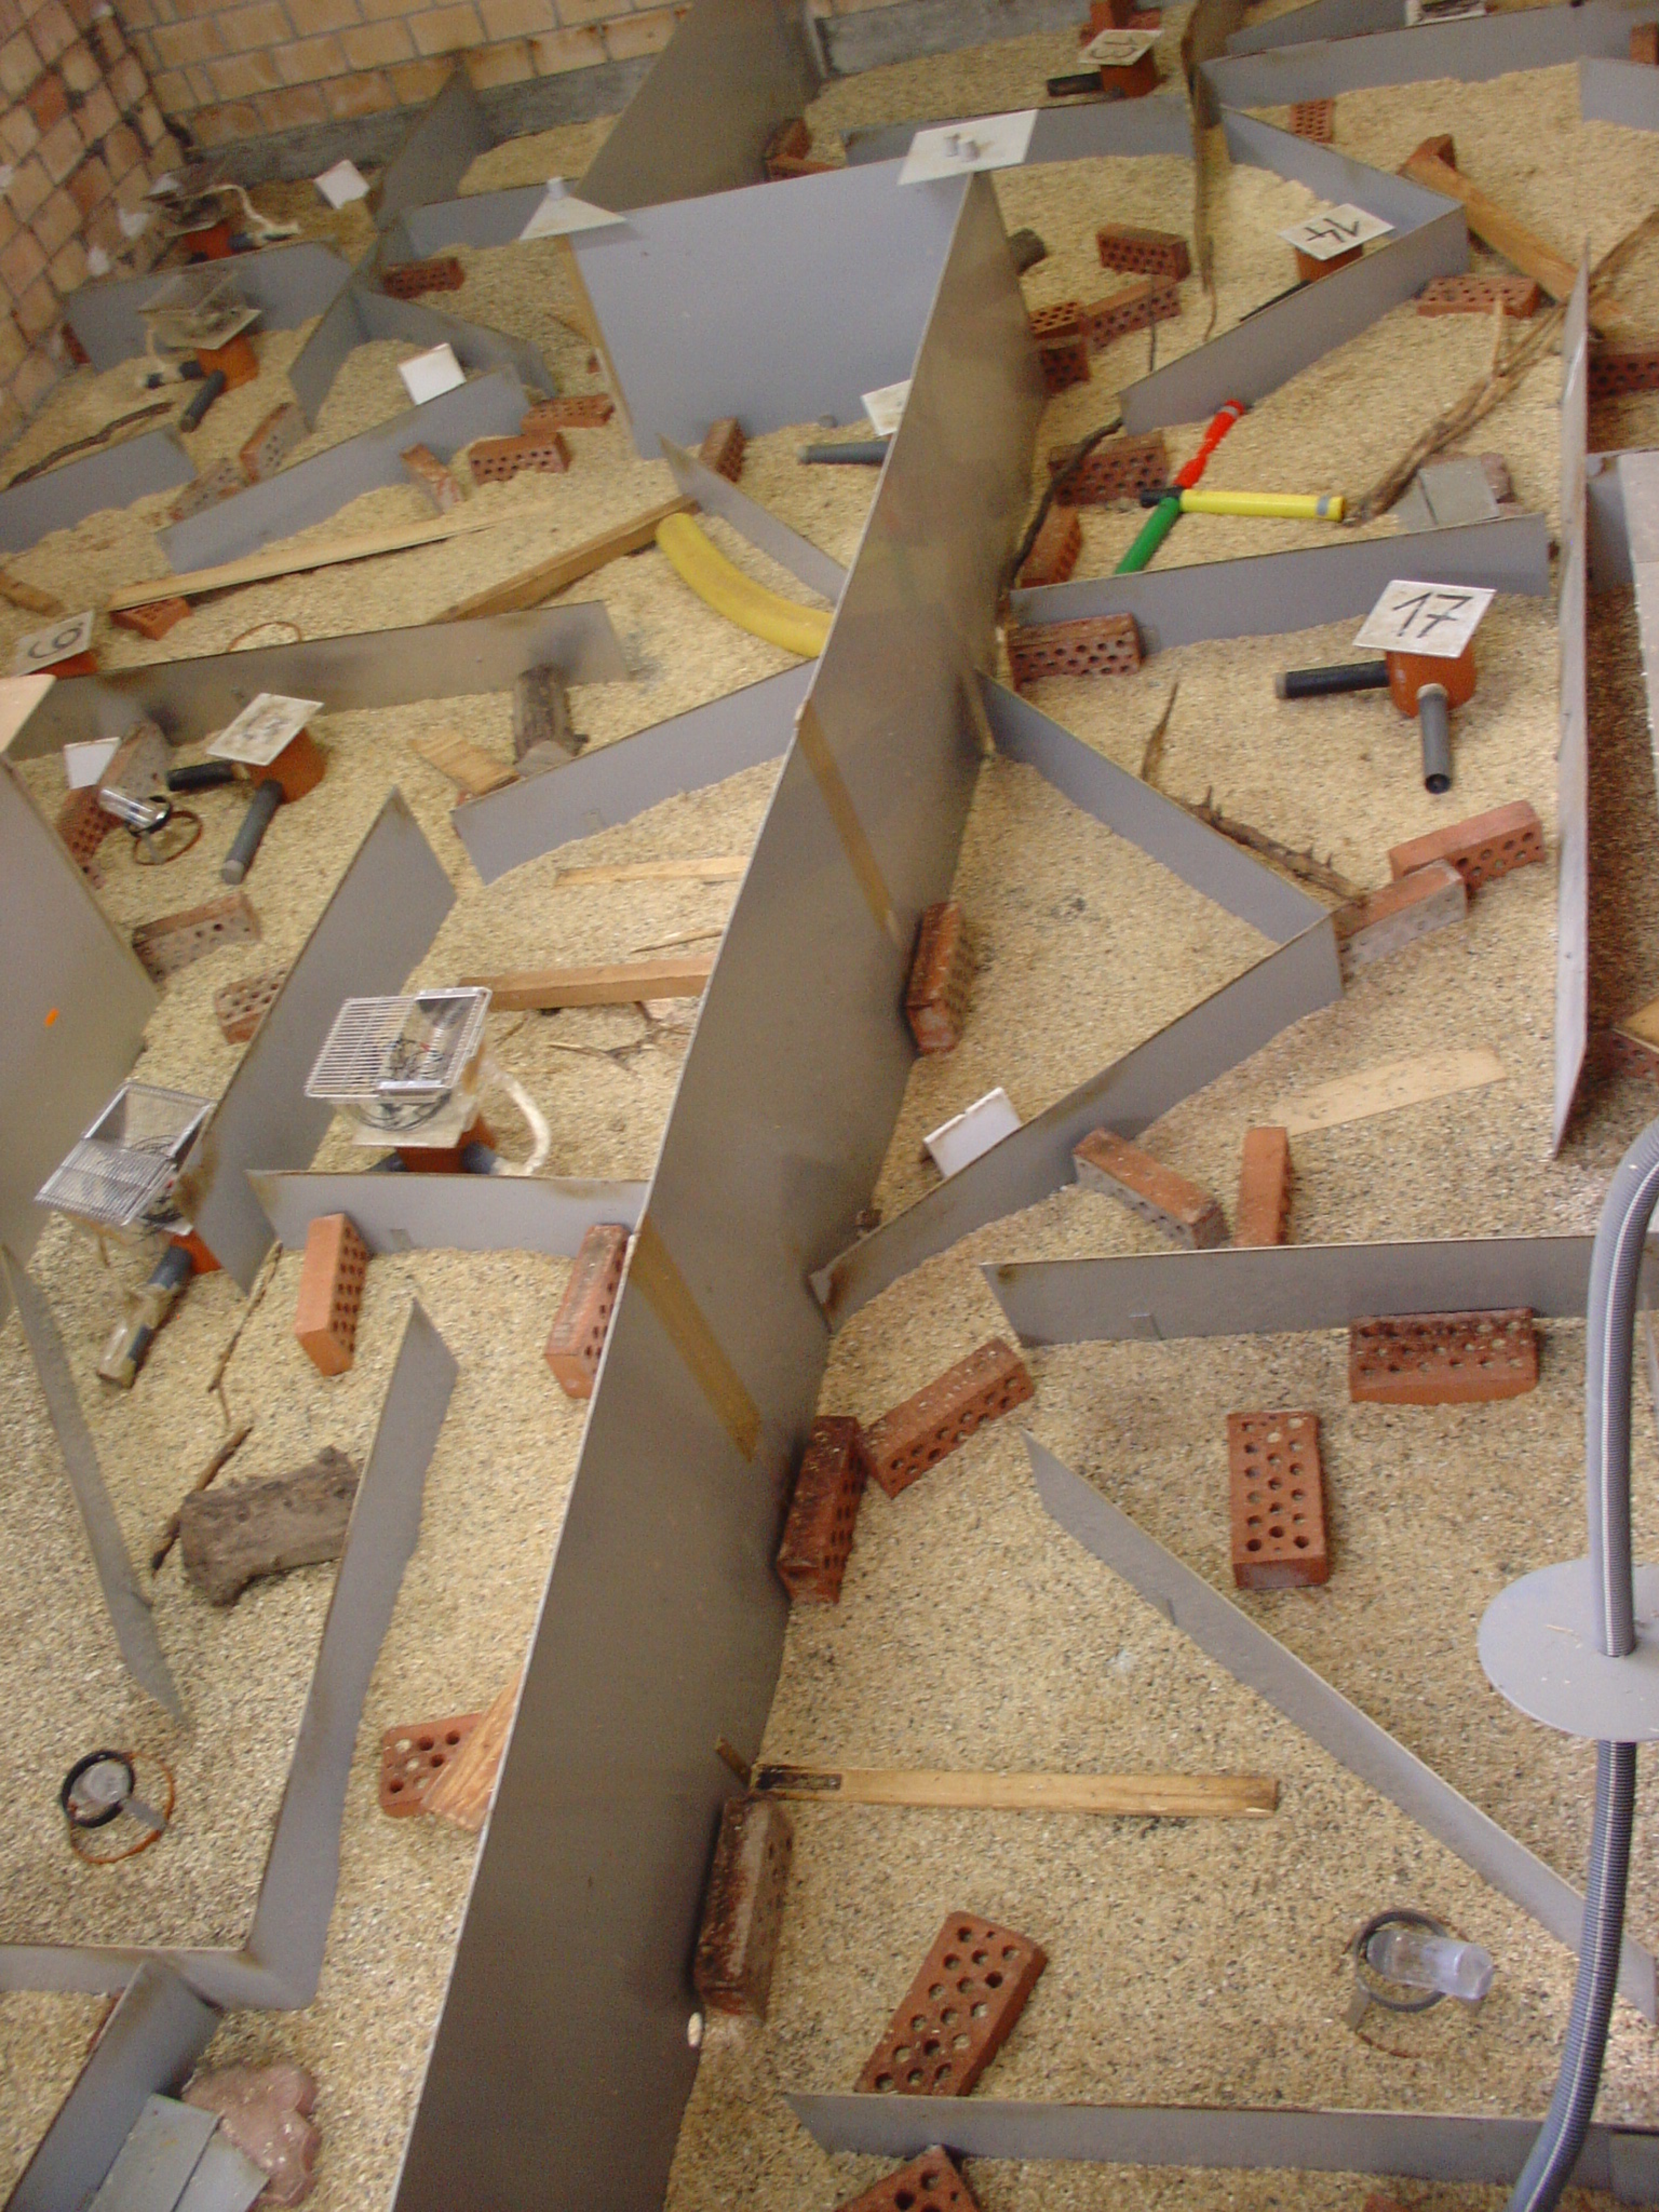
\includegraphics[width=0.7\textwidth]{assets/pdf/shed_overview.pdf}
  \caption[Interior of the barn]{Overview of the interior of the barn. Visible are the artificial nestboxes labeled with the box number on the white cover panel, the grey colored sector dividers and the accessory elements to structure the area.}
  \label{fig:shedoverview}
\end{center}
\end{figure}

\begin{sidewaysfigure}[htpb]
  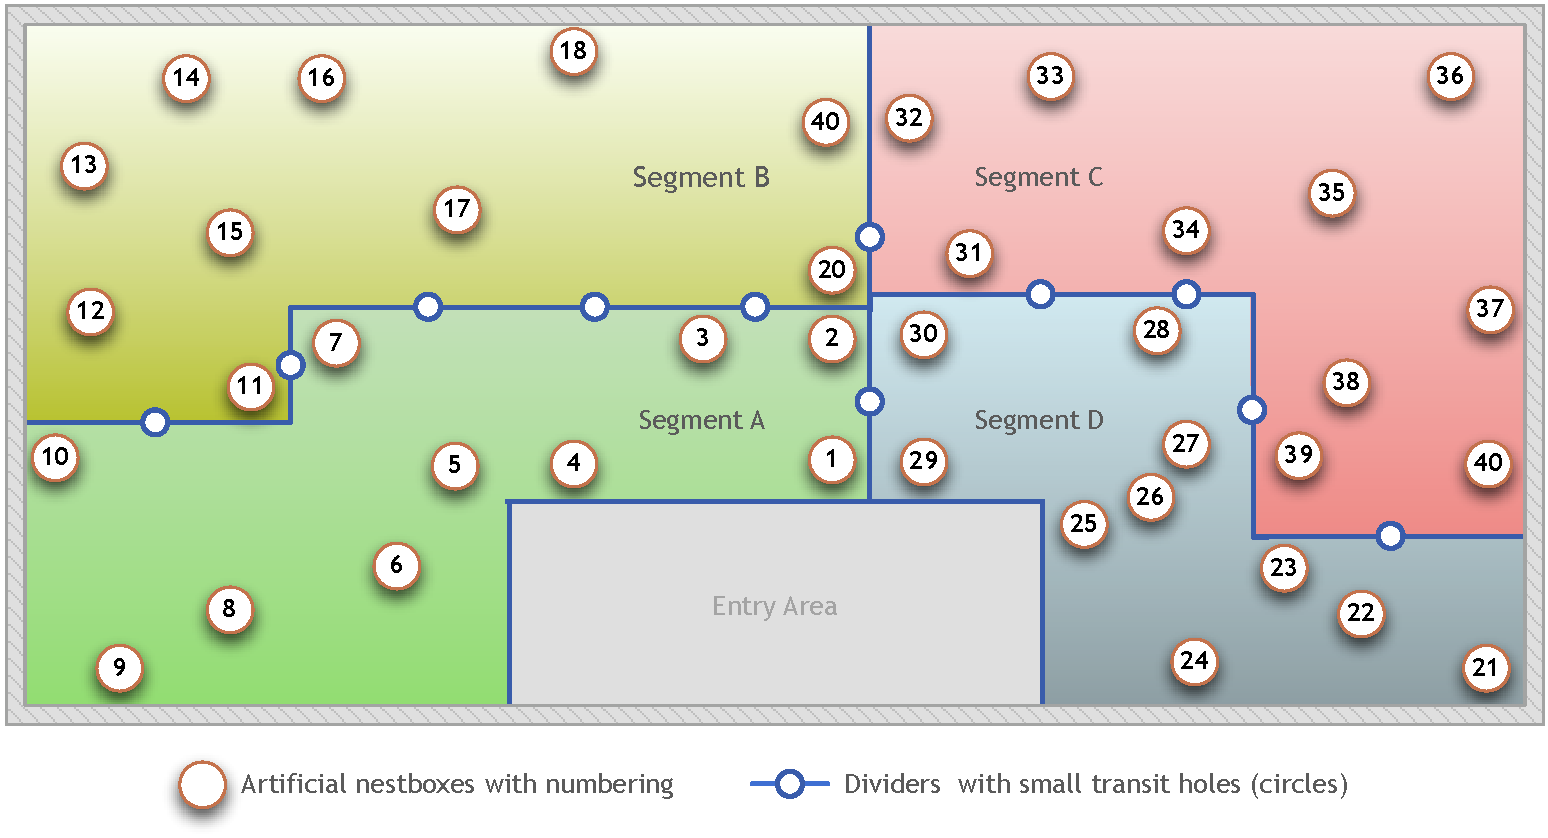
\includegraphics[width=\textwidth]{assets/pdf/shed_schema.pdf}
  \caption[Schema of the barn]{Schema of the barn including the box positions and the plastic walls dividing the area in the four segments. }
  \label{fig:barn_schema}
\end{sidewaysfigure}

% ===============================
% Data collection
% ===============================
% ===============================
% Data collection
% ===============================
\newpage
\section{Data}
\label{sec:datacollection}

When gathering data for behavioral analysis of different species, the observer usually tracks the position of one or several individuals over time. Additionally, pheno- and genotypical data is collected about each individual.

Spatial position is usually recorded by one or several persons. In this project however, data is collected by an antenna system (see section \ref{subsec:collectspatialpos}). Obviously, automated data collection has the advantage that data is recorded automatically around the clock every day.

To collect phenotypical data, so called \textit{population checks} (see \ref{subsec:dataattr} on page \pageref{subsec:dataattr} for details) are conducted every 6 to 8 weeks. During these checks, the mice are caught, measured, weighed (see section \ref{subsec:dataattr}) and - if not already present and the mouse has a weight of at least 18 grams - a \ac{RFID} (RFID) transponder is injected hypodermically (see figures \ref{fig:transponder} and \ref{fig:inject_rfid}). About 240 transponders are injected every year.

\begin{figure}[htpb]
\begin{center}
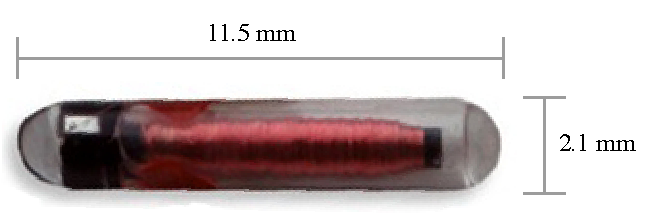
\includegraphics[width=0.5\textwidth]{assets/pdf/transponder.pdf}
  \caption[Trovan ID-100A Microtransponder]{A Trovan ID-100A Microtransponder. The transponder weighs 0.1 g and is coated with biocompatible glass. \footnotesize Picture courtesy of Trovan.}
  \label{fig:transponder}
\end{center}
\end{figure}
\begin{figure}[htpb]
\begin{center}
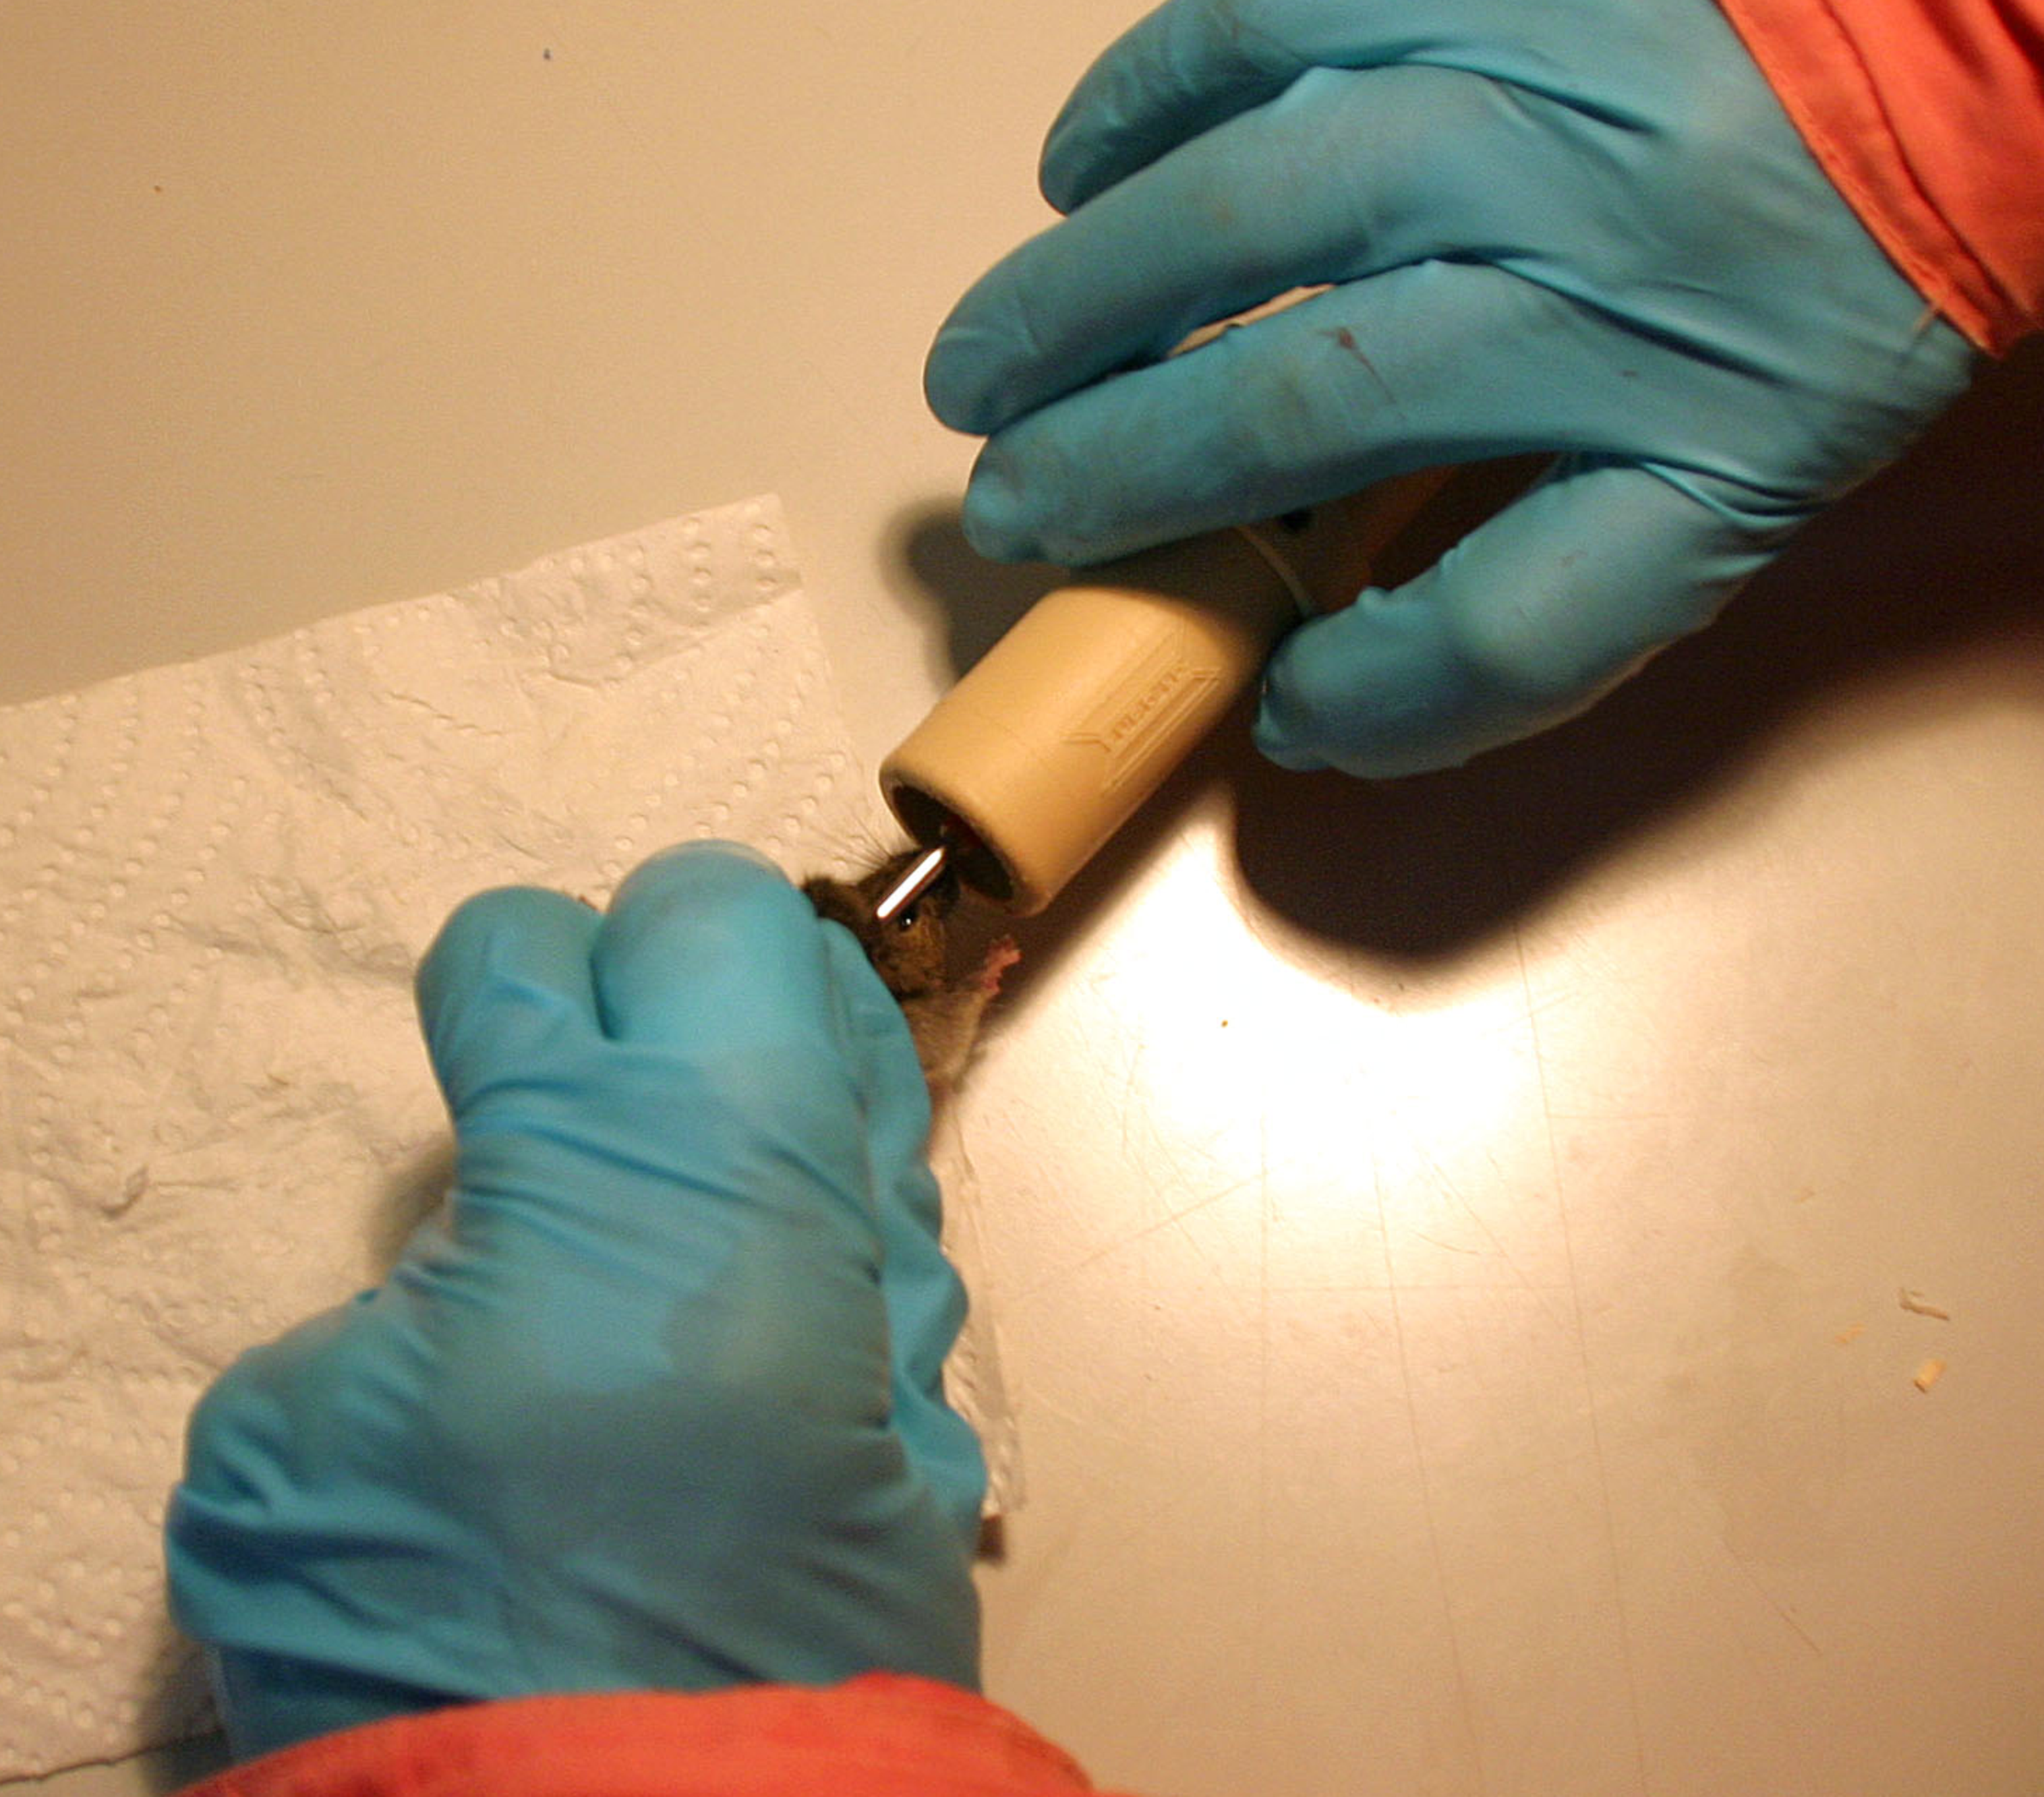
\includegraphics[width=0.5\textwidth]{assets/pdf/transponder_inject.pdf}
  \caption[Subcutaneous injection of an RFID transponder]{Subcutaneous injection of an RFID transponder.}
  \label{fig:inject_rfid}
\end{center}
\end{figure}

Furthermore, tissue samples are taken from the ear of each individual for genetic analysis. The genetic information provides an insight into the relatedness within the mice population and allows to compare specific genetic markers. Genotype information is not included in the data used for this thesis.

%----------------------------------------------
%Position / Time data
% ----------------------------------------------
\subsection{Collecting spatial position data}
\label{subsec:collectspatialpos}

To collect the spatial position data, a project-specific system has been by built by \textit{NewBehavior}, a company specialized in developing technical systems to study animal behavior.

The basic idea is to identify mice carrying an RFID transponder at specific locations. The locations where the identification occurs are the 40 artificial nestboxes distributed in the barn. 

An artificial nestbox consists of a cylinder, made of \ac{PVC}, with diameter and height of 15 cm and an entry tube made of \textit{Plexiglas}, which is about 20 to 25 cm long. Wrapped around the tube are two antennas with a coverage radius of 10 to 12 cm, capable of reading out the RFID transponders. Each antenna can be identified by an address which is set manually. To improve the antenna accuracy, the entry tube is bent 45 degrees to slow down the mice passing through. Figure \ref{fig:artNestbox} depicts a model of such an artificial nestbox.

\begin{figure}[htbp]	
\centering	
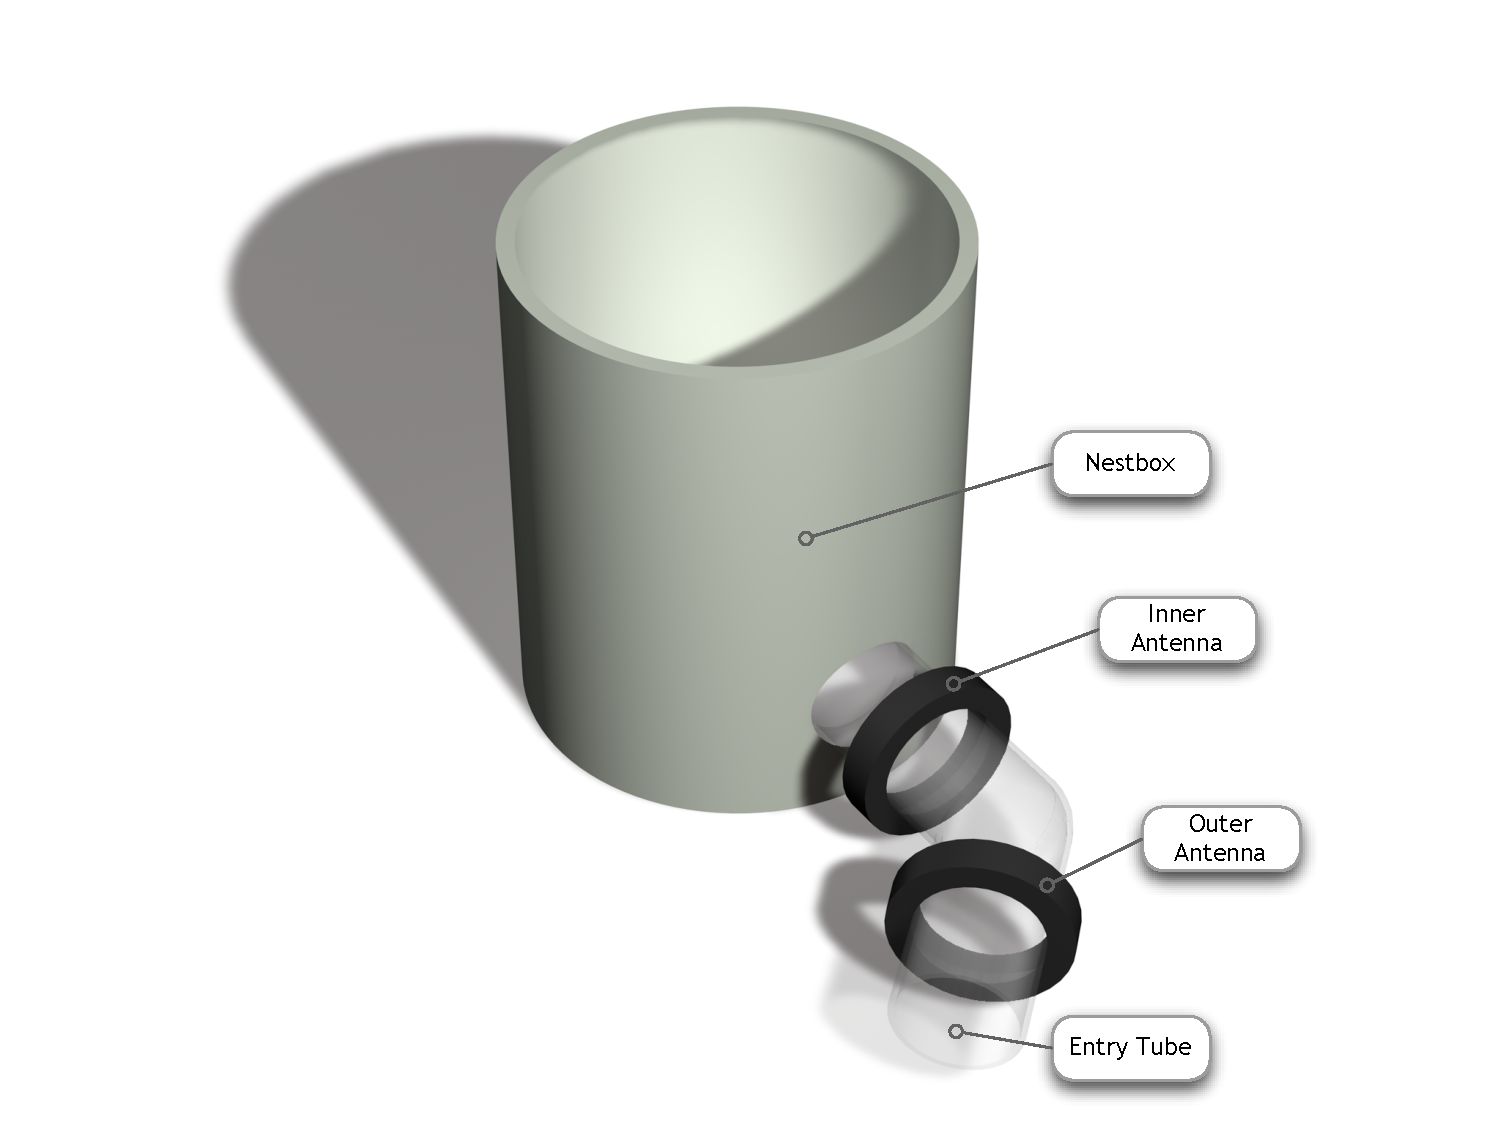
\includegraphics[width=0.75\textwidth]{assets/pdf/box_schema.pdf}	
\caption[3D-Model of an artificial nestbox]{3D-Model of an artificial nestbox with the two antennas wrapped around the entry tube.}
\label{fig:artNestbox}
\end{figure}

The RFID transponders used are passive, meaning that they do not include a battery. The antenna acts as a scanner, presenting an inductive field that excites the transponder within antenna range. This energy is used by the transponder to send its identification to the antenna. 

Therefore, whenever a mouse carrying a transponder passes by an antenna, its identification is recorded and sent to a central computer along with the antenna address. The computer then adds a time value to the received data before writing it to a text file. The structure of these text files containing the data is detailed in the next section.

\subsubsection{Data file format}
\label{subsubsec:datafileformat}
The data files are simple text files, where each line denotes an event registered by an antenna in the system. Every day the data file is saved, closed, and a new one is created automatically by the system.

There are to types of events: %Bullets! -tnetter 09/09/2009 15:35 % rico - how do put that in a list without a point at the end? 
\begin{mylist}
 \item The first type occurs if the antenna could identify a transponder. In such a case a line as shown in figure \ref{fig:dataset} is written to the data file. The id of the transponder is a unique, ten character wide, alphanumeric value
 \item The second type of event, for which the resulting data line looks as shown in Fig. \ref{fig:dataset_no_data}, occurs when a transponder enters or leaves the coverage area of an antenna
 \item 
\end{mylist}

\begin{figure}[!htbp]	
\centering	
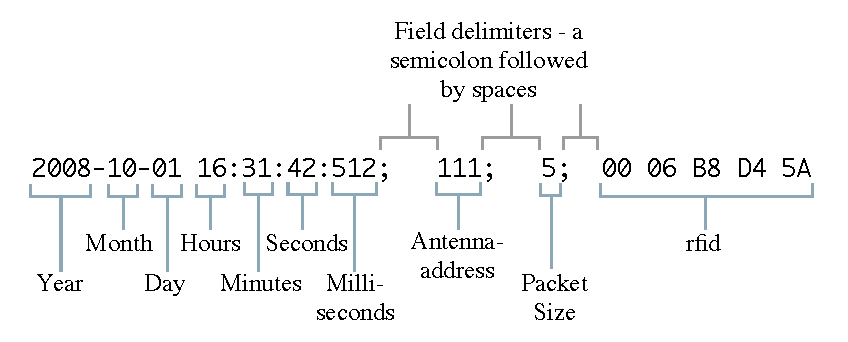
\includegraphics[width=0.6\textwidth]{assets/pdf/dataset.pdf}	
\caption[Dataset including an RFID transponder identification]{Typical dataset in a data file including an RFID transponder identification.}
\label{fig:dataset}
\end{figure}

\begin{figure}[!htbp]	
\centering	
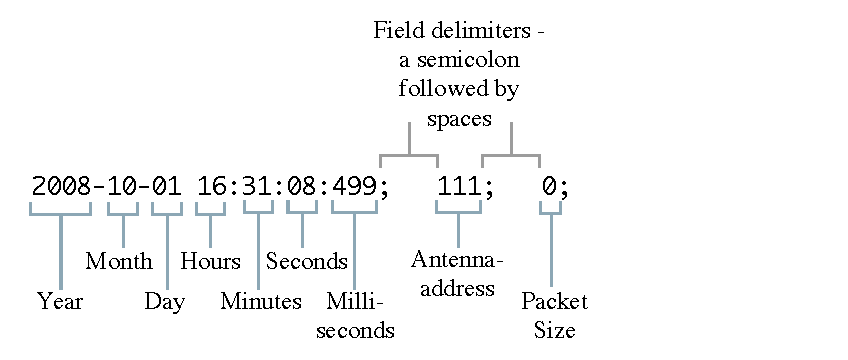
\includegraphics[width=0.6\textwidth]{assets/pdf/dataset_no_data.pdf}	
\caption[Dataset without RFID transponder identification]{Typical dataset in a data file without an RFID transponder identification.}
\label{fig:dataset_no_data}
\end{figure}

\needspace{9\baselineskip}
The following clipping and corresponding list show the data generated when a transponder passes by a nestbox. The events are explained in the subsequent list.  

\numcodestyle
\begin{lstlisting}[frame=none]
2008-10-01 16:31:08:499;   111;   0; 
2008-10-01 16:31:09:095;   113;   0; 
2008-10-01 16:31:42:512;   111;   5;  00 06 B8 D4 5A
2008-10-01 16:31:42:807;   113;   5;  00 06 B8 D4 5A
2008-10-01 16:31:43:619;   111;   0; 
2008-10-01 16:31:44:014;   113;   0;
\end{lstlisting}

The list numbering matches the line numbering of the clipping.  

\begin{condensed_enum}
  \item Transponder \textbf{enters coverage area} of the antenna with address \lstinline|111|.
  \item Transponder \textbf{enters coverage area} of the antenna with address \lstinline|113|.
  \item Transponder is \textbf{identified} as \lstinline|00 06 B8 D4 5A| at antenna with address \lstinline|111|.
  \item Transponder is \textbf{identified} as \lstinline|00 06 B8 D4 5A| at antenna with address \lstinline|113|.
  \item Transponder \textbf{leaves coverage area} of the antenna with address \lstinline|111|.
  \item Transponder \textbf{leaves coverage area} of the antenna with address \lstinline|113|. 
\end{condensed_enum}

Depending on the event type, the value of the packet size is either a \lstinline|0|, for events without a transponder identification value, or a \lstinline|5| if the transponder has been identified. For the data processing (see section \ref{sec:dataproc} on page \pageref{sec:dataproc}) only the datasets with a transponder identification are taken into account.

\subsubsection{Antenna addressing}
\label{subsubsec:addressing}

The antenna address is three digits long, composed of the box number it is attached to (first two digits) and the position at the entry tube of the box. Outer antennas have a \lstinline|1| as the last digit of the address, inner antennas a \lstinline|3| (e.g the antennas attached to box 11 are addressed 111 for the outer, 113 for the inner antenna, respectively). Needless to say, box numbers must be unique.

Unfortunately there are a few exceptions to that schema, as for a few antennas the correct addressing failed due to technical problems (see section \ref{subsec:problems}).

% \subsubsection{General system design and functionality}
% \label{subsubsec:generalsystem}
% 
% \begin{itemize}
%   \item Can-Bus
%   \item cable loop
%   \item rfid identification how
%   \item What happens in the boxes (boards) next to the antennas
%   \item How is can bus working/implemented
%   \item Where are the different cable loops (which antennas connected to a loop)
%   \item General system layout (cabling, protocols)
%   \item Programmed software
%   \item etc. 
% \end{itemize}

% ----------------------------------------------
%Data attributes
% ----------------------------------------------
\subsection{Collecting Data Attributes}
\label{subsec:dataattr}

During the \textit{population checks}, the whole barn, including all nestboxes, plastic pipes, and other structuring elements, is checked to collect mice attribute data according to the following procedure:

\begin{enumerate} 
\item Each box is opened and the following observations made:
\begin{mylist}
      \item \textbf{Mice in the box:} If adult mice are in the box, they get identified by their transponder, measured, and weighed. Furthermore we check whether the sex of the mouse has already been determined.  
      \item \textbf{Bedding:} Determine if the nestbox shows marks of use, like trampled bedding.
      \item \textbf{Nest:} Determine whether the nestbox contains an open or closed nest built by the mice out of hay or straw regularly provided in the barn.  
      \item \textbf{Pups:} Does the box contain pups, and if yes how many and what is their estimated age. 
      \item \textbf{Communal nest:} Check if two or more litters are reared in the box. 
    \end{mylist}
\item All the possible shelters, like planks and pipes, are checked for mice presence as well.
\end{enumerate}

% ----------------------------------------------
%storing Data
% ----------------------------------------------
\subsection{Data storage}
\label{subsec:datastorage}

This section details the design of the database. Data is stored in a \textit{MySQL}\footnote{\href{http://www.mysql.com/}{MySQL database}} database, which is  a \acf{RDBMS} (RDBMS). Figure \ref{fig:database_schema} on page \pageref{fig:database_schema} in the appendix shows an overview of all tables, including the data types\footnote{An overview of the MySQL data types can be found at: \url{http://dev.mysql.com/doc/refman/5.0/en/data-types.html}} of the columns and their relationship to columns in other tables.

Upon completion of a cascade of \ac{perl} scripts that process and extract information from the spatial position data in the data files, the resulting data is merged with the collected attribute data and is written to the tables as outlined in here. For details about the cascade refer to section \ref{sec:dataproc}. 

The tables can be split up in three different groups, depending of the sort of data they contain. 

\subsubsection{Processed data}

This group covers tables exclusively written to by the scripts in the import cascade. A diagram of the tables belonging to that group, as well as the relations between them, is shown in figure \ref{fig:processed_data_schema}. 

\begin{figure}[htpb]
\begin{center}
  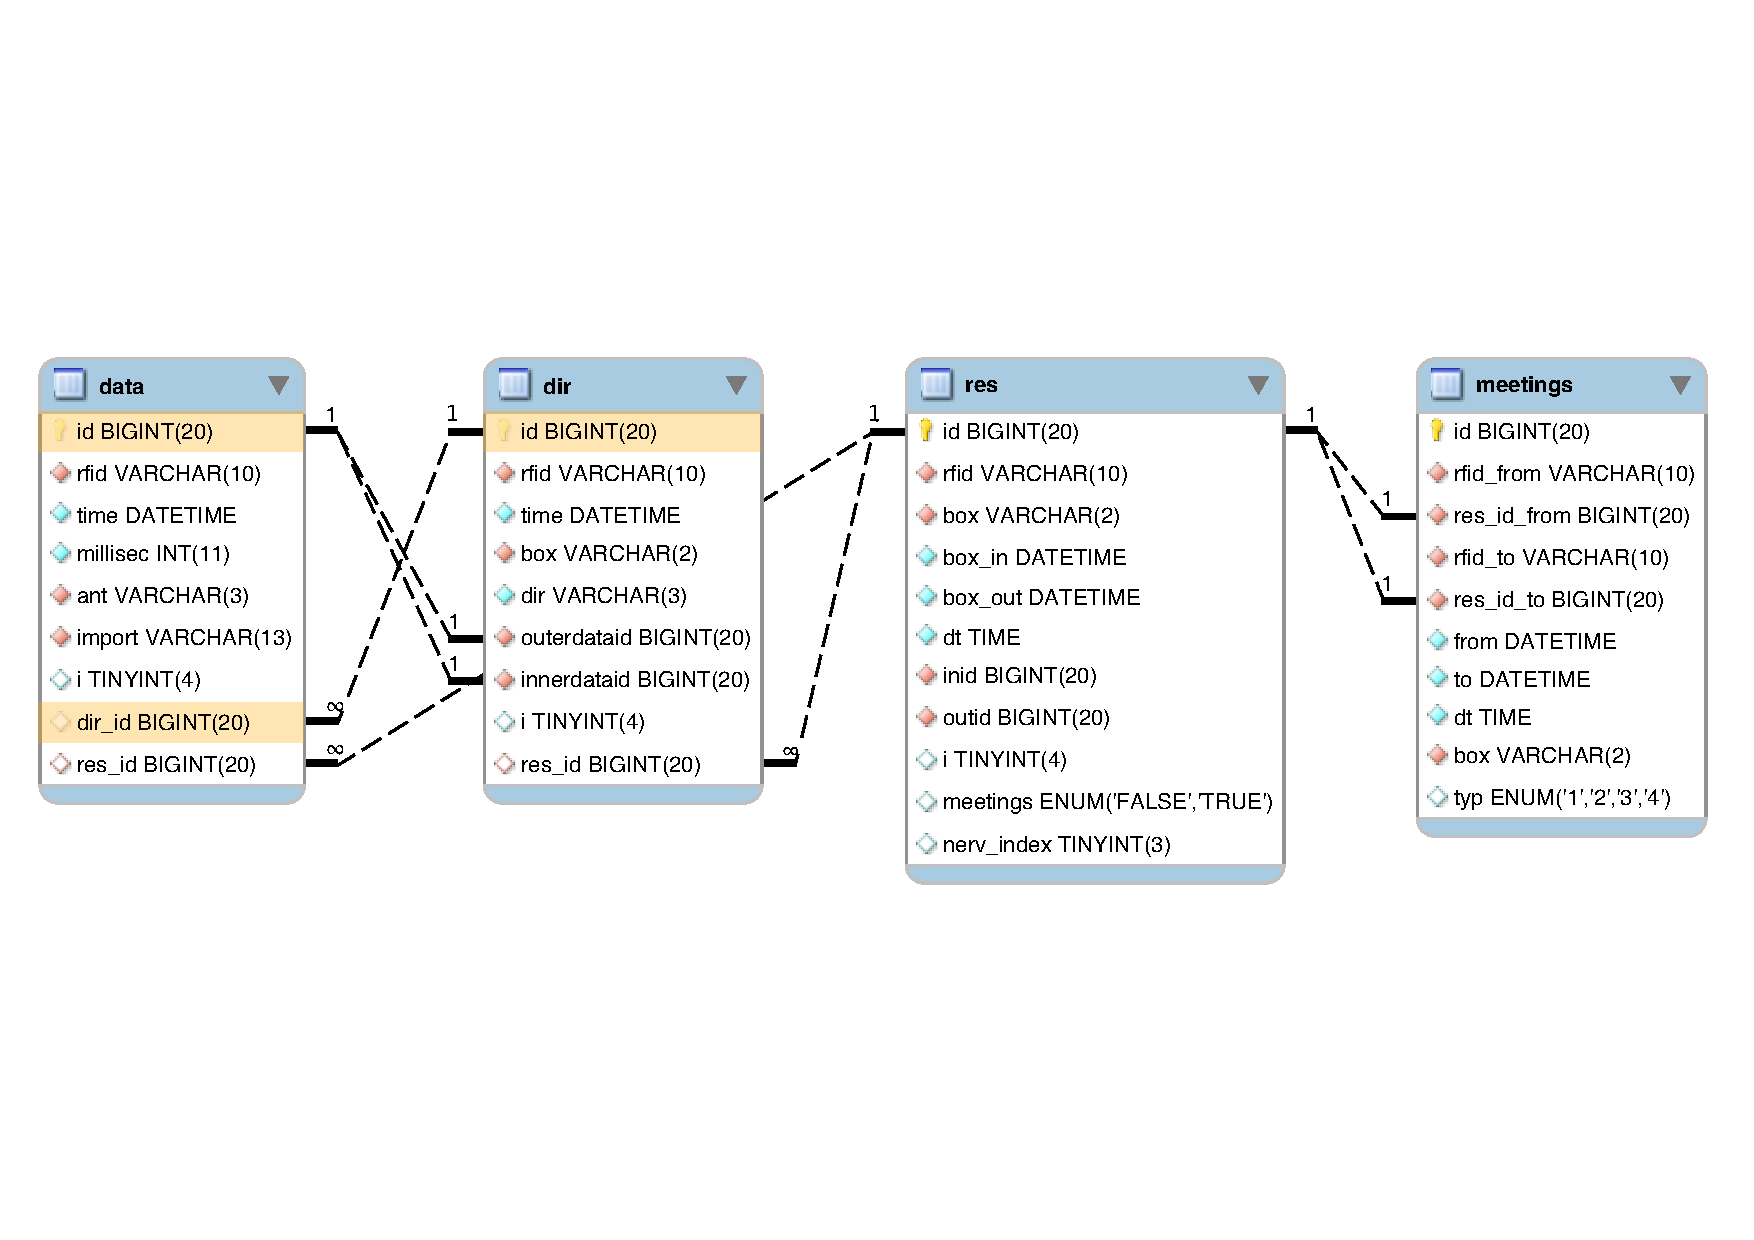
\includegraphics[width=\textwidth]{assets/pdf/processed_data_schema.pdf}
  \caption[Schema of database tables containing the processed data]{Schema of the database tables containing the processed spatial position data and the relations between them.}
  \label{fig:processed_data_schema}
\end{center}
\end{figure} 

\paragraph{data table}
\label{para:data_table}

A script (see section \ref{subsec:importing}) imports the data files written by the antenna system in the barn into the \lstinline|data| table.

Shown next is a row of the \lstinline|data| table followed by short explanation of the columns.

\codescript
\needspace{14\baselineskip}
\begin{lstlisting}[frame=none]

(first part of table row)
+---------+------------+---------------------+----------+
| id      | rfid       | time                | millisec |
+---------+------------+---------------------+----------+
| 7321019 | 00069B4D4D | 2009-02-07 00:51:56 |      173 |
+---------+------------+---------------------+----------+

(second part of table row)
+-----+---------------+------+--------+--------+
| ant | import        | i    | dir_id | res_id |
+-----+---------------+------+--------+--------+
| 121 | 09-0206155809 |    4 |  40102 |  10001 |
+-----+---------------+------+--------+--------+

\end{lstlisting}

\begin{mydesc}
  \item \lstinline|id| is a unique identifier of a dataset in this table. Such a unique identifier is normally used as target for a relation between columns of different tables and does not have any further meaning.
  \item \lstinline|rfid| is a transponder value. This value is a reference to a value in the \lstinline|id| column of the \lstinline|rfid| table (see section \ref{para:rfid_table}).
  \item \lstinline|time| and \lstinline|millsec| columns harbor the time the dataset has been recorded. Unfortunately the \textit{MySQL} \lstinline|DATETIME| data type does not include the milliseconds. Hence, these values have to be stored in a separate column.
  \item \lstinline|ant| denotes the antenna the data was recorded at. This value is a reference to a value in the \lstinline|id| column of the \lstinline|ant| table (see section \ref{para:ant_table}).
  \item \lstinline|import| is a reference to a dataset with an equivalent value of \lstinline|short| in the \lstinline|logs| table (see section \ref{para:logs_table}), simply unveils of which data file this dataset is part of.
  \item \lstinline|i| is an indicator if the dataset could be used in a \lstinline|direction result| and \lstinline|stay result| (see \ref{para:res_table}). Table \ref{tab:i_values} on page \pageref{tab:i_values} of the appendix gives an overview of the meaning of the \lstinline|i| values in the different tables.
  \item \lstinline|dir_id| is a reference to an \lstinline|id| in the \lstinline|dir| table, if that dataset could be used in a \textit{direction result}. Else, this value is \lstinline|NULL|\footnote{\textit{MySQL} sets the \lstinline|NULL| value to indicate a missing or unknown value.}.
  \item \lstinline|res_id| is a reference to an \lstinline|id| in the \lstinline|res| table, if that dataset could be used in a \textit{stay result}. Else this value is \lstinline|NULL|.
\end{mydesc}

\paragraph{dir table}
\label{para:dir_table}

Another script (see section \ref{subsec:dirres}) searches for matching pairs of datasets in the \lstinline|data| table which form a \textit{direction result}. When a mouse carrying a transponder passes the two antennas attached to the nestbox's entry tube, it is possible within a given time to determine if the mouse went in or out of that box. 

Shown next is a row of the \lstinline|dir| table followed by a short explanation of the columns.

\codescript
\needspace{14\baselineskip}
\begin{lstlisting}[frame=none]

(first part of table row)
+-------+------------+---------------------+-----+-----+
| id    | rfid       | time                | box | dir |
+-------+------------+---------------------+-----+-----+
| 40102 | 00069B4D4D | 2009-02-07 00:51:56 | 12  | in  |
+-------+------------+---------------------+-----+-----+

(second part of table row)
+-------------+-------------+------+--------+
| outerdataid | innerdataid | i    | res_id |
+-------------+-------------+------+--------+
|     7321019 |     7321020 |    4 |  10001 | 
+-------------+-------------+------+--------+
\end{lstlisting}

\begin{mydesc}
  \item \lstinline|id| and \lstinline|rfid| have the identical function as in the \lstinline|data| table.
  \item \lstinline|time| denotes the moment the the \lstinline|rfid| entered or left the \lstinline|box|.
  \item \lstinline|box| is a reference to a value in the \lstinline|id| column of the \lstinline|box| table (see section \ref{para:box_table}).
  \item \lstinline|dir| is either set to \lstinline|in| or \lstinline|out| and depicts the direction.
  \item \lstinline|outerdataid| and \lstinline|innerdataid| values can be used to backtrack the datasets in the \lstinline|data| table making up the \textit{direction result}. This is explained in detail in section \ref{subsec:dirres} on page \pageref{subsec:dirres}.
  \item \lstinline|i| is an indicator if the direction result could be used in a \textit{stay result} (see \ref{para:res_table}). Table \ref{tab:i_values} on page \pageref{tab:i_values} of the appendix gives an overview of the meaning of the \lstinline|i| values in the different tables.
  \item \lstinline|res_id| is a reference to an \lstinline|id| in the \lstinline|res| table, if that dataset could be used in a \textit{stay result}. Else this value is \lstinline|NULL|.
\end{mydesc}

\paragraph{res table}
\label{para:res_table}

When two \textit{direction results} are found (one with a \lstinline|dir| value of \lstinline|in| and the other with a \lstinline|dir| value of \lstinline|out|, as well as matching \lstinline|rfid| and \lstinline|box| values), they form a so called \textit{stay result}.

Shown next is a row of the \lstinline|res| table followed by a short explanation of the columns.

\codescript
\needspace{14\baselineskip}
\begin{lstlisting}[frame=none]

(first part of table row)
+-------+------------+-----+---------------------+---------------------+
| id    | rfid       | box | box_in              | box_out             |
+-------+------------+-----+---------------------+---------------------+
| 10001 | 00069B4D4D | 12  | 2009-02-07 00:51:56 | 2009-02-07 00:52:01 |
+-------+------------+-----+---------------------+---------------------+

(second part of table row)
+----------+-------+---------+------+----------+------------+
| dt       | inid  | outid   | i    | meetings | nerv_index |
+----------+-------+---------+------+----------+------------+
| 00:00:05 | 40102 | 7321021 |    4 | TRUE     |          1 | 
+----------+-------+---------+------+----------+------------+

\end{lstlisting}

\begin{mydesc}
\item \lstinline|id|, \lstinline|rfid| and \lstinline|box| were already explained for the previous tables, and have the same function in this table.
\item \lstinline|box_in| and \lstinline|box_out| denote the arrival and departure times of an \lstinline|rfid| in a \lstinline|box|.
\item \lstinline|dt| denotes the duration of the result, equal to the time elapsed between \lstinline|box_in| and \lstinline|box_out|.
\item \lstinline|inid| and \lstinline|outid| can be used to backtrace the datasets in the \lstinline|dir| or \lstinline|data| table making up the \textit{stay result}.
\item \lstinline|i| is either \lstinline|3| or \lstinline|4| and indicates the type of result. This distinction is explained in section \ref{subsec:stayres}.
\item \lstinline|meetings| is set to \lstinline|true| when the result set has been analyzed for meetings (see next paragraph and section \ref{subsec:meetingres} for details about the \textit{meeting results}).
\item \lstinline|nerv_index| gives an idea about how \textit{nervous} the mouse was when it stayed in the box. Details about this value can be found in section \ref{subsec:stayres} as well.
\end{mydesc}

\paragraph{Meetings table}
\label{para:meetings_table}

In this work, an event is termed a \textit{meeting}, if \textit{stay results} of different mice in the same box show a temporal overlap. The meeting data is written to the \lstinline|meetings| table.

Shown next is a row of the \lstinline|meetings| table followed by a short explanation of the columns.

\codescript
\needspace{14\baselineskip}
\begin{lstlisting}[frame=none]

(first part of table row)
+--------+------------+-------------+------------+-----------+
| id     | rfid_from  | res_id_from | rfid_to    | res_id_to |
+--------+------------+-------------+------------+-----------+
| 302635 | 0006CD478F |      596630 | 0006CC7962 |    596100 | 
+--------+------------+-------------+------------+-----------+

(second part of table row)
+---------------------+---------------------+----------+-----+------+
| from                | to                  | dt       | box | typ  |
+---------------------+---------------------+----------+-----+------+
| 2009-03-27 16:58:36 | 2009-03-27 17:01:00 | 00:02:24 | 13  | 1    |
+---------------------+---------------------+----------+-----+------+
\end{lstlisting}

\begin{mydesc}
\item \lstinline|id| is again the unique identifier.
\item \lstinline|rfid_from| and \lstinline|rfid_to| denote the two participating RFID's (mice) of the \textit{meeting result}.
\item \lstinline|res_id_from| points to the \lstinline|id| of the \textit{stay result} from the \lstinline|rfid_from|, and the \lstinline|res_id_to| to the one of the \lstinline|rfid_to|. This allows to look up the \textit{stay results} making up this \lstinline|meeting result|.
\item \lstinline|from|, \lstinline|to| and \lstinline|dt| declare the meeting's start and end times, as well as duration.
\item \lstinline|box| contains the reference to an \lstinline|id| in the \lstinline|box| table (see section \ref{para:box_table}).
\item The different values of the \lstinline|typ| column are detailed in section \ref{subsec:meetingres}.
\end{mydesc}

\subsubsection{System members data}
\label{subsubsec:system_members_tables}

This group encloses the tables which contain information about the RFID's (transpondered mice) as well as the antennas and boxes.

Figure \ref{fig:system_members} shows an overview of the tables within this group plus the relations between the table columns. 

\begin{figure}[htpb]
\begin{center}
  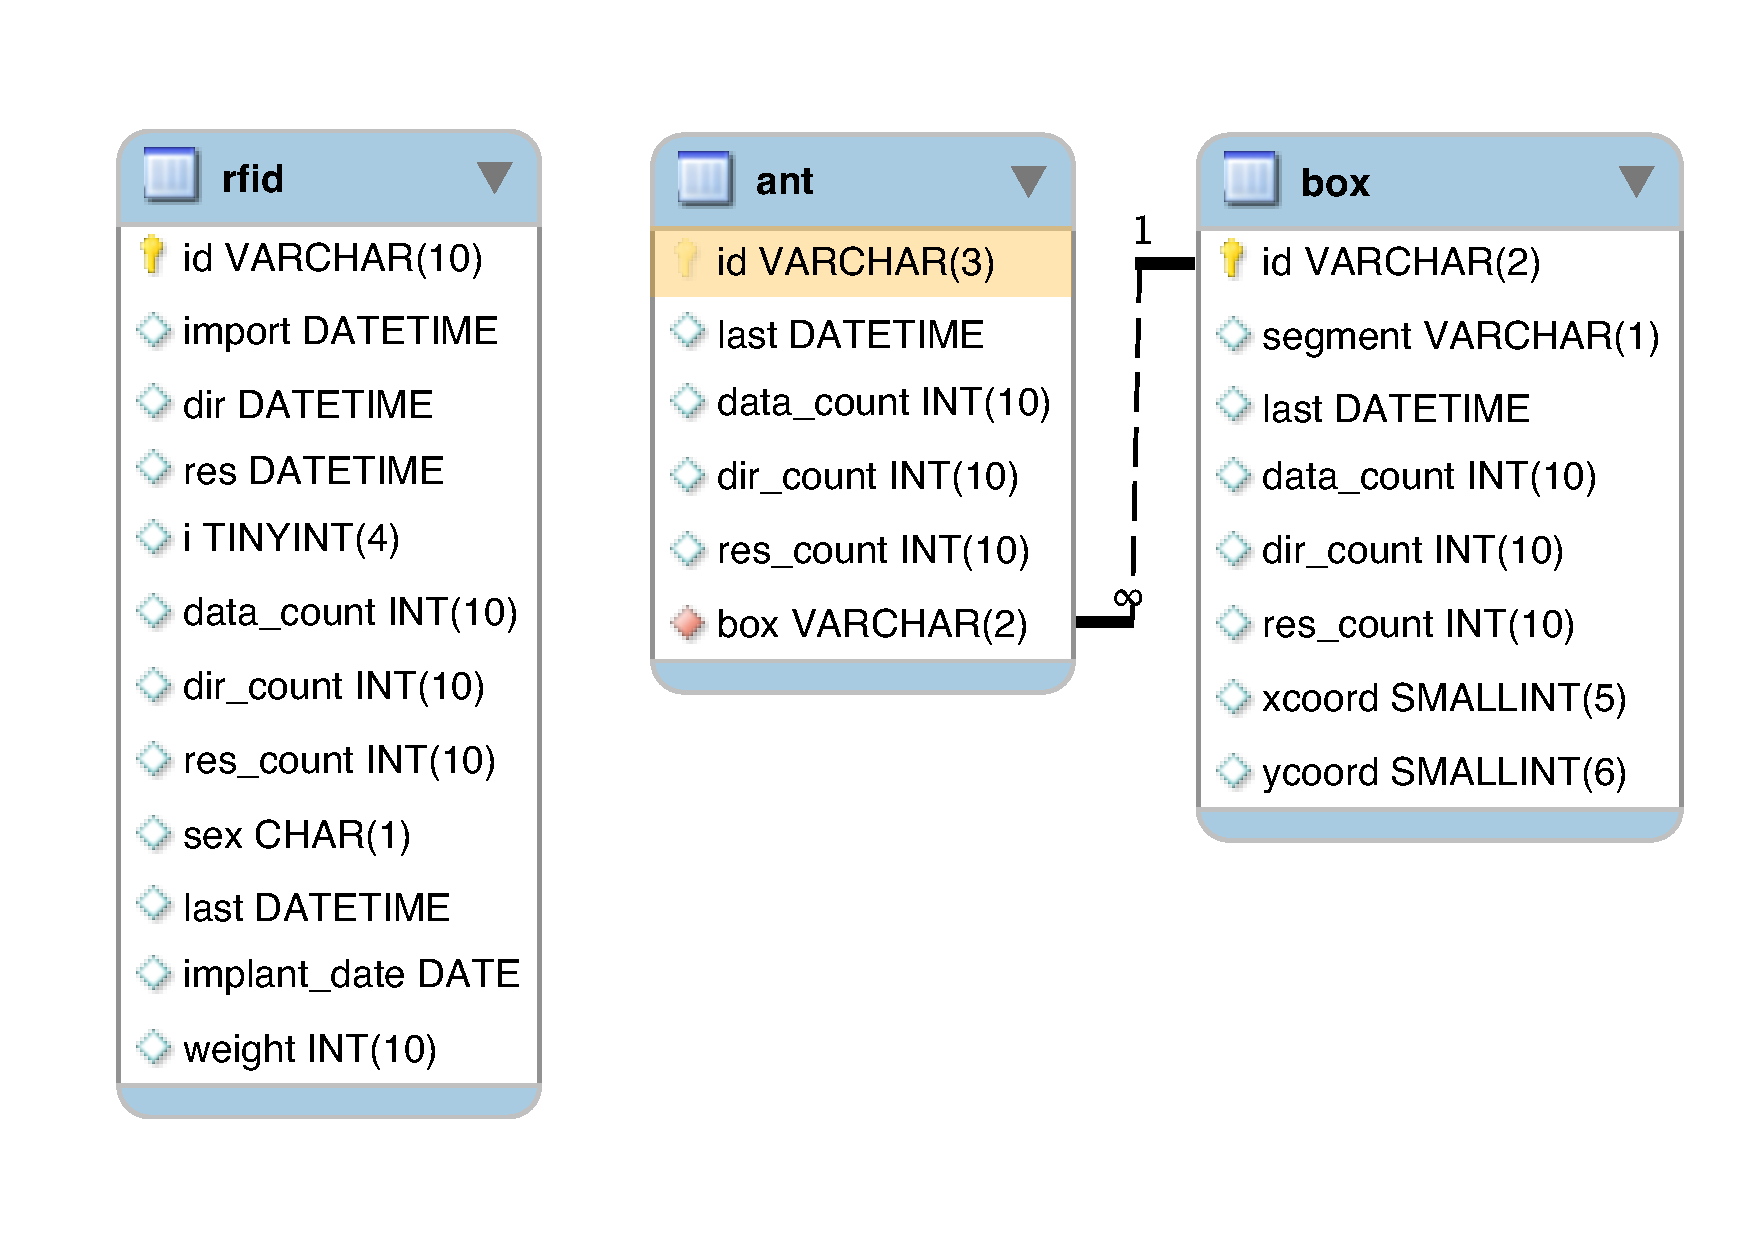
\includegraphics[width=0.75\textwidth]{assets/pdf/system_members_schema.pdf}
  \caption[Schema of database tables containing the system member data]{Schema of the database tables containing the \textit{system members} data.}
  \label{fig:system_members}
\end{center}
\end{figure}

\paragraph{rfid table}
\label{para:rfid_table}

All the RFID's ever recorded by the system, including their corresponding attribute data, are stored in the \lstinline|rfid| table.

Shown in the next listing is a row of the \lstinline|rfid| table followed by short a explanation of the columns.
\codescript
\needspace{14\baselineskip}
\begin{lstlisting}[frame=none]

(first part of table row)
+------------+------+------------+-----------+-----------+
| id         | i    | data_count | dir_count | res_count |
+------------+------+------------+-----------+-----------+
| 0006955EED |    3 |          1 |         0 |         0 |
+------------+------+------------+-----------+-----------+

(second part of table row)
+------+---------------------+--------------+--------+
| sex  | last                | implant_date | weight |
+------+---------------------+--------------+--------+
| m    | 2007-08-29 23:35:41 | 2007-08-28   |   18.0 |
+------+---------------------+--------------+--------+

\end{lstlisting}

\begin{mydesc}
\item \lstinline|id| is the unique, 10 character wide, alphanumeric RFID transponder identification.
\item \lstinline|i| is is a helper value used in the data import procedure. It is \lstinline|0| if new data for the transponder has been imported, \lstinline|2| if the data is searched for \textit{direction results} and \lstinline|3| if the data has been searched for \textit{stay results}.
\item \lstinline|data_count| contains the sum of datasets in the \lstinline|data| table.
\item \lstinline|dir_count| contains the sum of datasets in the \lstinline|direction| table.
\item \lstinline|res_count| contains the sum of datasets in the \lstinline|results| table.
\item \lstinline|sex| denotes the gender of the mouse, when known.
\item \lstinline|last| points to the maximum value in the \lstinline|time| column of the \lstinline|data| table for this mouse, which is just the last time the transponder has been recorded by the antenna system.
\item \lstinline|implant_date| holds the date of the RFID tag's hypodermic injection.
\item \lstinline|weight| contains a decimal number with the weight of the mouse in grams.
\end{mydesc}

\paragraph{box table}
\label{para:box_table}

The box table contains all the information about the 40 nestboxes. 

Shown next is a row of the \lstinline|box| table followed by a short explanation of the columns.
\codescript
\needspace{14\baselineskip}
\begin{lstlisting}[frame=none]

(first part of table row)
+----+---------+---------------------+------------+
| id | segment | last                | data_count |
+----+---------+---------------------+------------+
| 01 | A       | 2009-03-27 16:38:59 |     122439 | 
+----+---------+---------------------+------------+

(second part of table row)
+-----------+-----------+--------+--------+
| dir_count | res_count | xcoord | ycoord |
+-----------+-----------+--------+--------+
|     44389 |      9824 |    246 |    708 | 
+-----------+-----------+--------+--------+

\end{lstlisting}

\begin{mydesc}
\item \lstinline|id| is the unique 2 character wide box identification.
\item \lstinline|segment| points to the segment (A, B, C or D) the box is located in.
\item The meaning of the \lstinline|last|, \lstinline|data_count|, \lstinline|dir_count| and \lstinline|res_count| columns was already explained in the \lstinline|rfid| table.
\item \lstinline|xcoord| and \lstinline|ycoord| denote the position of the nestbox in the barn. The x-axis stands for the entrance wall and the y-axis for  the side wall to the left of the entrance. The coordinate values are stored in centimeters. 
\end{mydesc}

\paragraph{ant table} 
\label{para:ant_table}

The ant table contains all the information about the 80 antennas. 

Shown next is a row of the \lstinline|ant| table followed by a short explanation of the columns.
\codescript
\needspace{14\baselineskip}
\begin{lstlisting}[frame=none]
+-----+---------------------+------------+-----------+-----------+-----+
| id  | last                | data_count | dir_count | res_count | box |
+-----+---------------------+------------+-----------+-----------+-----+
| 011 | 2009-03-27 16:38:59 |      54220 |     46099 |     19648 | 01  | 
+-----+---------------------+------------+-----------+-----------+-----+

\end{lstlisting}

\begin{mydesc}
\item \lstinline|id| is the unique 3 character wide antenna address.
\item The meaning of the \lstinline|last| \lstinline|data_count|, \lstinline|dir_count| and \lstinline|res_count| columns was already explained in the \lstinline|rfid| table.
\item \lstinline|box| points to the \lstinline|id| value in the \lstinline|box| table, the antenna is attached to.
\end{mydesc}

\subsubsection{Auxiliary tables}
\label{subsubsec:auxiliary_tables}

Tables in this group contain data about the imported data files, and precalculated values to improve the performance when browsing the data using the graphical user interface (which is introduced in section \ref{subsec:dataexp}).

Figure \ref{fig:auxiliary_tables} shows an overview of the tables within this group. 


\begin{figure}[htpb]
\begin{center}
  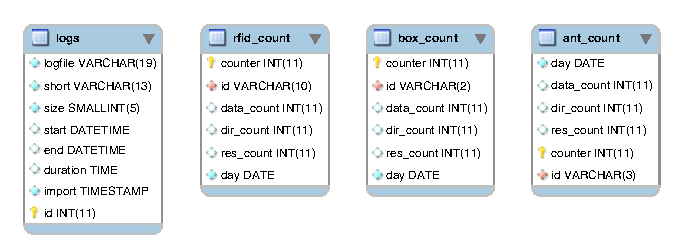
\includegraphics[width=0.75\textwidth]{assets/pdf/auxiliary_tables_schema.pdf}
  \caption[Schema of database tables containing the auxiliary data]{Schema of the database tables containing the auxiliary data.}
  \label{fig:auxiliary_tables}
\end{center}
\end{figure}

\paragraph{logs table}
\label{para:logs_table} 

The \lstinline|logs| table contains information about the imported data files.

Shown next is a row of the \lstinline|logs| table followed by a short explanation of the columns.

\codescript
\needspace{14\baselineskip}
\begin{lstlisting}[frame=none]
(first part of table row)
+-----+---------------------+---------------+------+---------------------+
| id  | logfile             | short         | size | start               |
+-----+---------------------+---------------+------+---------------------+
| 608 | 20090326_170750.txt | 09-0326170750 | 1660 | 2009-03-26 17:07:51 |
+-----+---------------------+---------------+------+---------------------+

(second part of table row)
+---------------------+----------+---------------------+
| end                 | duration | import              |
+---------------------+----------+---------------------+
| 2009-03-27 17:07:40 | 23:59:49 | 2009-04-12 01:03:01 | 
+---------------------+----------+---------------------+

\end{lstlisting}

\begin{mydesc}
\item \lstinline|id| is the unique identifier of dataset.
\item The original filename of the data file is stored in the \lstinline|logfile| column.
\item \lstinline|short| values are a kind of code made up from parts of the data filename. This column was important at the beginning of the project, when we had to import data files with another file format.
\item \lstinline|size| contains the filesize, in bytes, of the data file.
\item \lstinline|start| and \lstinline|end| indicate the file's first and last record timestamps.
\item \lstinline|duration| is simply the period between the \lstinline|start| and \lstinline|end| values.
\item \lstinline|import| is the data import into \lstinline|data| completion timestamp.
\end{mydesc}

\paragraph{RFID\_count, box\_count, ant\_count}
\label{para:counts}

These three tables contain the per day data counts for transponders (\lstinline|rfid_count|), boxes (\lstinline|box_count|), and antennas (\lstinline|ant_count|). They are only needed by the user interface to speed up data browsing.

Shown next is a row of the \lstinline|rfid_count|, \lstinline|box_count|, \lstinline|ant_count| tables followed by a short explanation of the columns.

\codescript
\needspace{14\baselineskip}
\begin{lstlisting}[frame=none]
(row of table rfid_count)
+---------+------------+------------+------------+-----------+-----------+
| counter | id         | day        | data_count | dir_count | res_count |
+---------+------------+------------+------------+-----------+-----------+
|     999 | 0006B9C5E8 | 2008-07-14 |         10 |         4 |         2 | 
+---------+------------+------------+------------+-----------+-----------+


(row of table box_count)
+---------+----+------------+------------+-----------+-----------+
| counter | id | day        | data_count | dir_count | res_count |
+---------+----+------------+------------+-----------+-----------+
|     999 | 10 | 2008-07-31 |        259 |       114 |        39 | 
+---------+----+------------+------------+-----------+-----------+


(row of table ant_count)
+---------+-----+------------+------------+-----------+-----------+
| counter | id  | day        | data_count | dir_count | res_count |
+---------+-----+------------+------------+-----------+-----------+
|     999 | 121 | 2008-07-19 |        196 |       174 |        47 | 
+---------+-----+------------+------------+-----------+-----------+


\end{lstlisting}

\begin{mydesc}
\item \lstinline|counter| is the unique dataset identifier.
\item \lstinline|id| contains the \lstinline|id| value of the transponder, the box or the antenna.
\item \lstinline|day| points to the day the table row holds the data counts for.
\item \lstinline|data_count|, \lstinline|dir_count| and \lstinline|res_count| contain the per day counts for the datasets, the \textit{direction results} and the \textit{stay results}.
\end{mydesc}

\subsection{Efficiency and problems of the antenna system}
\label{subsec:problems}

Unfortunately the problems with the antenna system are diverse such as antenna drop outs, broken laptop or cable connections chewed by mice, to name just a few. Some of these problems could be solved.

However, one of the biggest problem is that the readings at the antennas are not as reliable as expected. This is clearly visible by looking at the efficiency of the system , measured by comparison of theoretical and actual number of \textit{direction} and \textit{say results}. 

From the 5th of April 2007 to the 27th of March 2009, approximately 8 million datasets (table \lstinline|data|)  
have been collected. Theoretically we would get around 4 million \textit{direction results}. The actual number of \textit{direction  results} is 2.9 million. The exact percentage is 71.16\%.

In the next step, two \textit{direction results} should create a \textit{stay result}. The script which searches for the \textit{stay results} could find 1.5  results in the 3 million \textit{direction results}, but finds around one million. More exactly  68.25\%. Most likely these low numbers are an effect of missed antenna readings.
 
Normally, an antenna reads the RFID tag 10 times to increase a reading's reliability. The antenna system in the barn, however, reads the RFID only 3 times, as the time that a tagged mouse spends within antenna range is usually short. We can partly understand the impact of shortened sampling duration by looking at the \lstinline|rfid| table. The table contains 4605 different transponder id's, whereby only 1014 have been sampled over 10 times. The other 3546 RFID's are most probably a result of a phenomenon called \textit{bit flipping}.

The following listing shows an excerpt of a data file, where a RFID tag is identified as \lstinline|00 05 B8 D2 70| on line two, but as \lstinline|00 06 B8 E2 70| on the other lines. 

\numcodestyle
\needspace{5\baselineskip}
\begin{lstlisting}[frame=none]
2007-11-25 10:09:12:906;   381;   5;  00 06 B8 E2 70
2007-11-25 10:09:16:529;   381;   5;  00 05 B8 D2 70
2007-11-25 10:09:16:932;   381;   5;  00 06 B8 E2 70
2007-11-25 10:09:19:950;   381;   0; 
2007-11-25 10:09:20:253;   381;   5;  00 06 B8 E2 70
\end{lstlisting}

The first four digits of the transponder identification represent the manufacturer's serial number. The manufacturer sold us only RFID's from the \lstinline|00 06| series. Because of this we can conclude that line two is a read error. Still, this transponder has been read 53 times between November 2007 and May 2008, but none of the readings could be used to form a \textit{direction result}. Assuming that this is not a singular case, we get many of these false readings which lead to a low subsequent data processing yield. 

Furthermore, for some antennas the address could not be set properly. In one case two antennas even sent the same address, so that distinction of the data is impossible. The workaround for this problem is to find an unused address which we are able to set, and map it to the desired address during data import (see section \ref{subsec:importing}).   

\subsection{Data access}
\label{subsec:dataccess}

Most of the mainly used relational databases offer \ac{SQL} (SQL) to manage and retrieve data. However, SQL is not easy to learn and use, lacks built-in export functionality to file formats such as \textit{Microsoft Excel}, and does not offer the possibility to visualize data. We therefore provide a feature-rich and intuitive \acf{GUI} (GUI) to facilitate exploration, visualization, and data export. A presentation of the GUI can be found in section \ref{sec:dataaccessandexp}.

% ===============================
% Data processing
% ===============================
% ===============================
% Data processing
% ===============================
\newpage
\section{Data Processing}
\label{sec:dataproc}

Figure \ref{fig:app_design_perl} shows an overview of the different parts involved in the data importing and analysis process. The \ac{perl} scripts which are reading data from and writing data to the database build the main part of this framework\footnote{The directories in which the scripts, modules and files are located, are listed in table \ref{tab:directories_and_files_overview} on page \pageref{tab:directories_and_files_overview}.}.

\begin{figure}[htpb]
\begin{center}
  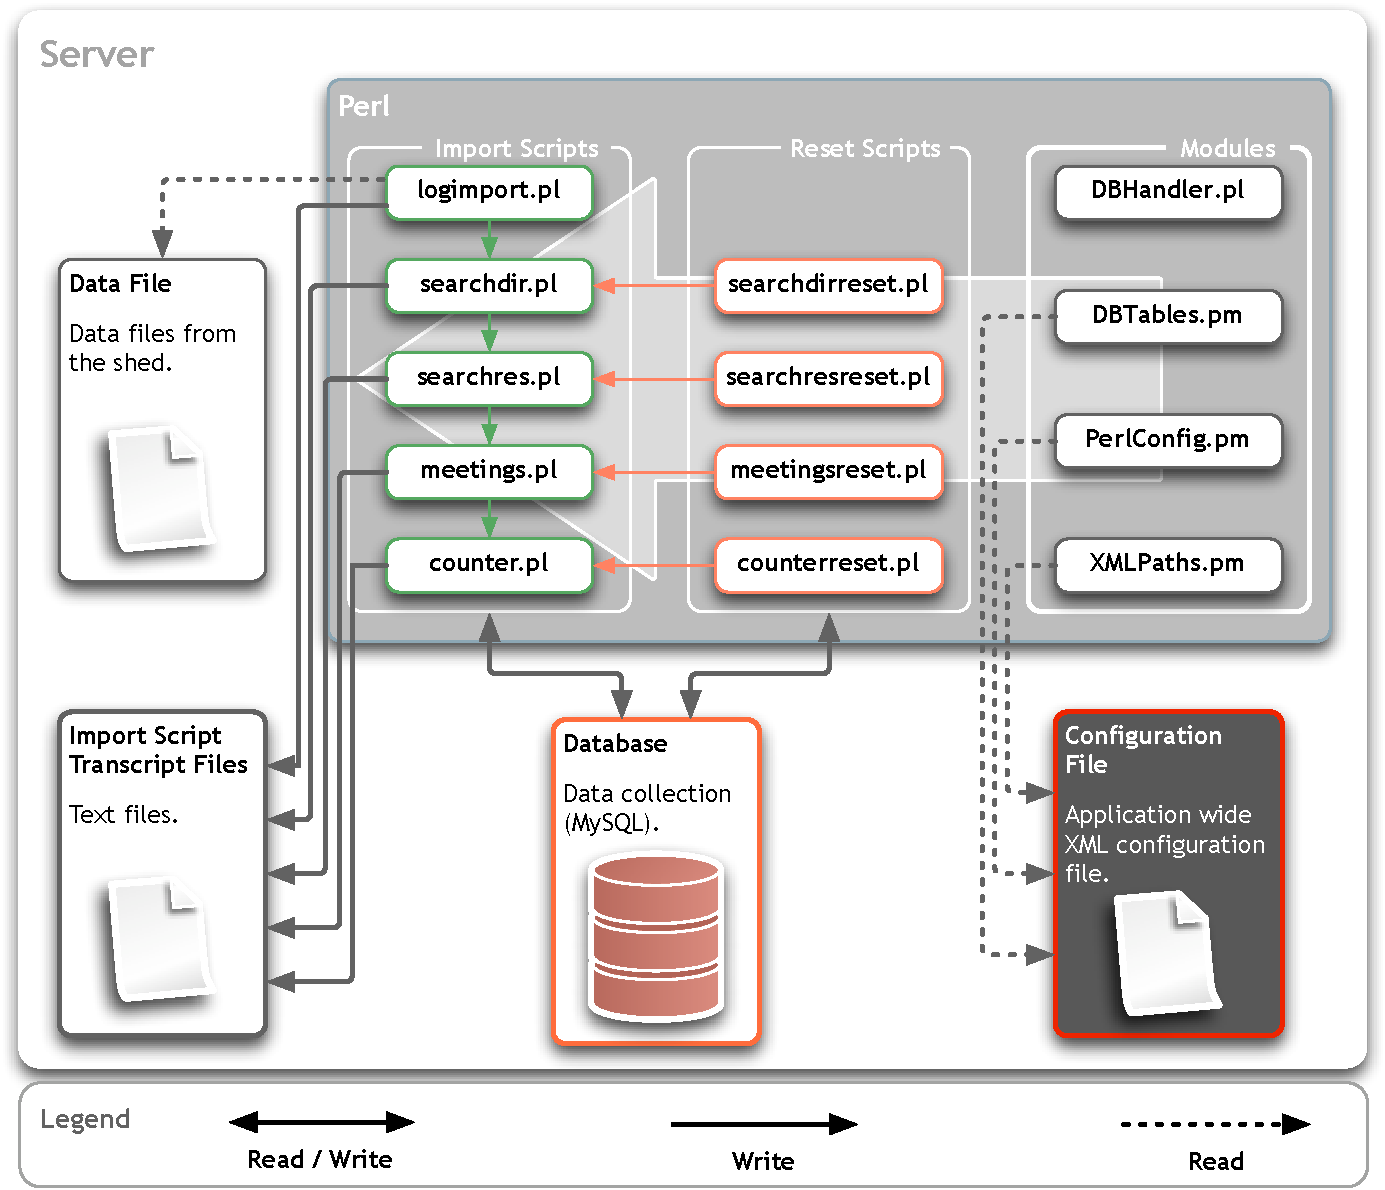
\includegraphics[width=\textwidth]{assets/pdf/app_design_perl.pdf}
  \caption[Data processing overview]{Overview of the parts involved in the data processing.}
  \label{fig:app_design_perl}
\end{center}
\end{figure}

The \textit{Import Scripts} run in a cascade, beginning with the \lstinline|logimport.pl| script, which is reading the data files from the shed, and ending with the \lstinline|counter.pl| script (indicated in figure \ref{fig:app_design_perl} by the green arrows). Each of these scrips writes a transcript file to make their progress traceable. Upon completion of the cascade, the data files are imported and stored in the respective tables as outline in section \ref{subsec:datastorage} on page \pageref{subsec:datastorage}.

A scheduled, daily task checks for new data files uploaded to the server and starts the cascade if needed\footnote{For details about this topic see appendix \ref{app:import_schedule} on page \pageref{app:import_schedule}.}.

The \textit{Reset Scripts} set the database back to a state from where the import cascade can be rerun,  starting with the corresponding import script (indicated in figure \ref{fig:app_design_perl} by the orange arrows). If, for example, the \lstinline|searchdirreset.pl| has been executed, the import cascade can be started with the \lstinline|searchdir.pl| script\footnote{It is recommended to start the import cascade by using the import BASH scripts. This is explained in appendix \ref{app:import_schedule} on page \pageref{app:import_schedule}.}.

The \textit{Modules} read out the configuration and make it available for the import and reset scripts (indicated in figure \ref{fig:app_design_perl} by the large grey arrow with the white border). The whole configuration for the application is stored in an XML file. The part of configuration file accountable for the perl part is shown in appendix \ref{app:configperl} on page \pageref{app:configperl}. As the perl scripts are heavily interacting with the database, the database configuration part of the configuration is read as well by some of the \textit{Modules}\footnote{The database configuration is shown and explained in appendix \ref{app:configdb} on page \pageref{app:configdb}.}. 

\subsection{Importing}
\label{subsec:importing}

The \lstinline|logimport.pl| extracts the spatial position data from the data files and writes it to the \lstinline|data| table \footnote{The \lstinline|data| table structure is descriped section \ref{para:data_table} on page \pageref{para:data_table}.}.

Prior to the data extraction, the  script creates a backup of the actual database\footnote{The configuration for the backup is explained in appendix \ref{app:configperl} on page \pageref{app:configperl}.}. Subsequently the data is extracted from the data files and written to the database. 

As mentioned in section \ref{subsubsec:problems} on page \pageref{subsubsec:problems}, some of the antennas could not be addressed properly. Therefore, the script has to catch these exceptional values and convert them to the designated ones\footnote{See listing \ref{lst:antenna_adress_conversions} on page \pageref{lst:antenna_adress_conversions} for the detailed conversions.}.  

\subsection{Direction Results}
\label{subsec:dirres}

The \lstinline|searchdir.pl| script searches for matching pairs of antenna readings in the \lstinline|data| table, which build a \textit{direction result}. A pair matches if,

\begin{mylist}
\item the transponder identification values of the two readings is the same,
\item time difference in seconds between the two readings is not greater then the value set as the \lstinline|<antennaInterval>| value \footnote{See appendix \ref{app:configperl} on page \pageref{app:configperl}.} in the configuration, 
\item and the readings originate from the two different antennas attached to a box.  
\end{mylist}

This is exactly the order this script searches for \textit{direction results}. The findings are written to the \lstinline|dir| table\footnote{The \lstinline|dir| table structure described in sction \ref{para:dir_table} on page \pageref{para:dir_table}}. The value for the \lstinline|time| field of the \textit{direction result} is always taken from the antenna reading at the outer antenna.

If the \lstinline|<antennaInterval>| has been changed, the \lstinline| searchdirreset.pl| needs to be executed followed by the scripts in the import cascade starting with the \lstinline|searchdir.pl| script \footnotemark[14]. 

\subsection{Stay Results}
\label{subsec:stayres}

The \lstinline|searchres.pl| aims to find matching \textit{direction results} in the \lstinline|dir| table, which build a \textit{stay results}.

A pair matches if,

\begin{mylist}
\item the transponder identification values of the two \textit{direction results} are the same
\item the \lstinline|direction| values of the \textit{direction results} are oppositional
\item and the \textit{direction results} are recorded at the same box.
\end{mylist}

or,

\begin{mylist}
\item the transponder identification values of a \textit{direction result} with a \lstinline|direction| value of \lstinline|in| and an unused (=could not be used for a \textit{direction result}) dataset from the \lstinline|data| table recorded at an outer antenna, are the same
\item and belong to the same box.
\end{mylist}

In the former case, it is written to the \lstinline|res| table as a \textbf{type 3} result in the latter case a \textbf{type 4} result \footnote{See section \ref{para:res_table} on page \pageref{para:res_table} for details about the \lstinline|res| table.}. 

Additionaly, the script has to handle the temporal overlaps of stay results. Since, the antenna system is not working perfect (see section \ref{subsubsec:problems}), if we let the script search for all possible \textit{stay results}, we get situations as illustrated in figures \ref{fig:result_overlap} and \ref{fig:result_overlap_single}. The antenna system must have missed readings, but we have no clue about the exact moment.

\begin{figure}[htpb]
\begin{center}
  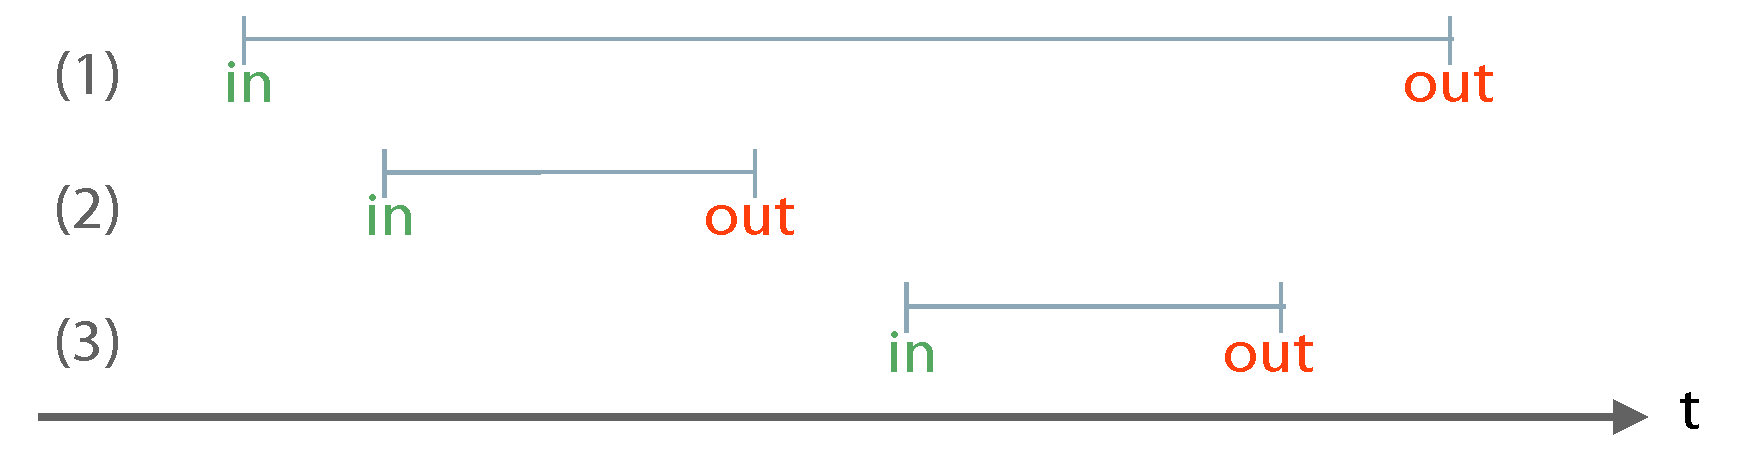
\includegraphics[width=0.75\textwidth]{assets/pdf/result_overlaps_schema.pdf}
  \caption[Multiple result overlap illustration]{Illustration of a possible result overlap situation, where one \textit{stay result} overlaps many others.}
  \label{fig:result_overlap}
\end{center}
\end{figure}

\begin{figure}[htpb]
\begin{center}
  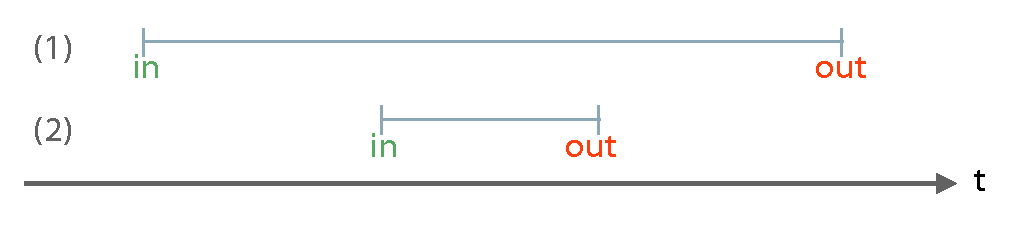
\includegraphics[width=0.75\textwidth]{assets/pdf/result_overlaps_single_schema.pdf}
  \caption[Single result overlap illustration]{Illustration of a possible result overlap situation, where a \textit{stay result} overlaps another.}
  \label{fig:result_overlap_single}
\end{center}
\end{figure}

A mouse is termed \textit{nervous}, when she has been read at the inner antenna of the box but not at the outer antenna. The mouse is out of the box only when she is read at the outer antenna of the box.

\subsection{Meeting Results}
\label{subsec:meetingres}

Aim of the script / step.
Describing code, rules used to calculate the association results.

% ===============================
% Data exploration
% ===============================
% ===============================
% Data exploration
% ===============================
\newpage
\section{Accessing and exploring the Data }
\label{sec:dataaccessandexp}

As seen in the previous sections, the amount of available data in the database is enormous. In the field of computer technology, the process of scanning such a huge pool of data for \textit{potentially interesting} sets of data is called \textit{data mining}. What's \textit{potentially interesting} completely depends on the researchers intention. Therefore, a multitude of filter and visualization options should be available, to facilitate the data exploration. Once a desired set of data has been identified, one should be able to export that data for further analysis. 

\subsection{Introducing miceminer}
\label{subsec:dataexp}

The \textit{miceminer} application intends to meet exactly these requirements. Written entirely in \textit{Flex}\footnote{Adobe Flex is a software development kit released by Adobe Systems for the development and deployment of cross-platform rich Internet applications based on the Adobe Flash platform \cite{wiki:flex}.}, the application runs within every web browser with the $Flash^{\copyright}$ plug-in version 9 or above installed. Thus, the software is cross platform compatible, meaning that it runs on every operating system for which the $Flash^{\copyright}$ player is available. 

Furthermore, the \textit{miceminer} application doesn't need to be installed on every computer, but is stored on a computer accessible over the internet, which is called a server. Every time the application is accessed, it gets downloaded to the inquiring computer, which is called the client. This has the comfortable consequence, that each user always uses the latest version.

Additionaly, \textit{Flex} offers convincing tools to build interactive user interfaces and, in counjunction with third party software, dependable ways to retrieve data from a database. Compared to \textit{Java}\footnote{Java is a programming language.[\ldots] Java application can run on any Java virtual machine (JVM) regardless of computer architecture\cite{wiki:java}.}, which has a immense \ac{API}, the \ac{API} offered by \textit{Flex} is appropriate for our needs.

Additional information about the \textit{miceminer} project, including screencasts which show how to use teh application, \ac{API} documentation, source code and links to resources used, can be found on the project homepage at \href{http://zool-miceminer.uzh.ch/}{http://zool-miceminer.uzh.ch}. 

\subsection{Interface}
\label{subsec:miceminer_interface}

This section gives a very short introduction to the user interface. User help can be found on the project homepage. Furthermore, all of the components contain a help button in the upper right corner. Clicking on this button reveals the help text for the component.

Figure \ref{fig:interface_overview} shows a screenshot of the \textit{miceminer} interface and identifies the main parts. 

\begin{figure}[!ht]
\begin{center}
  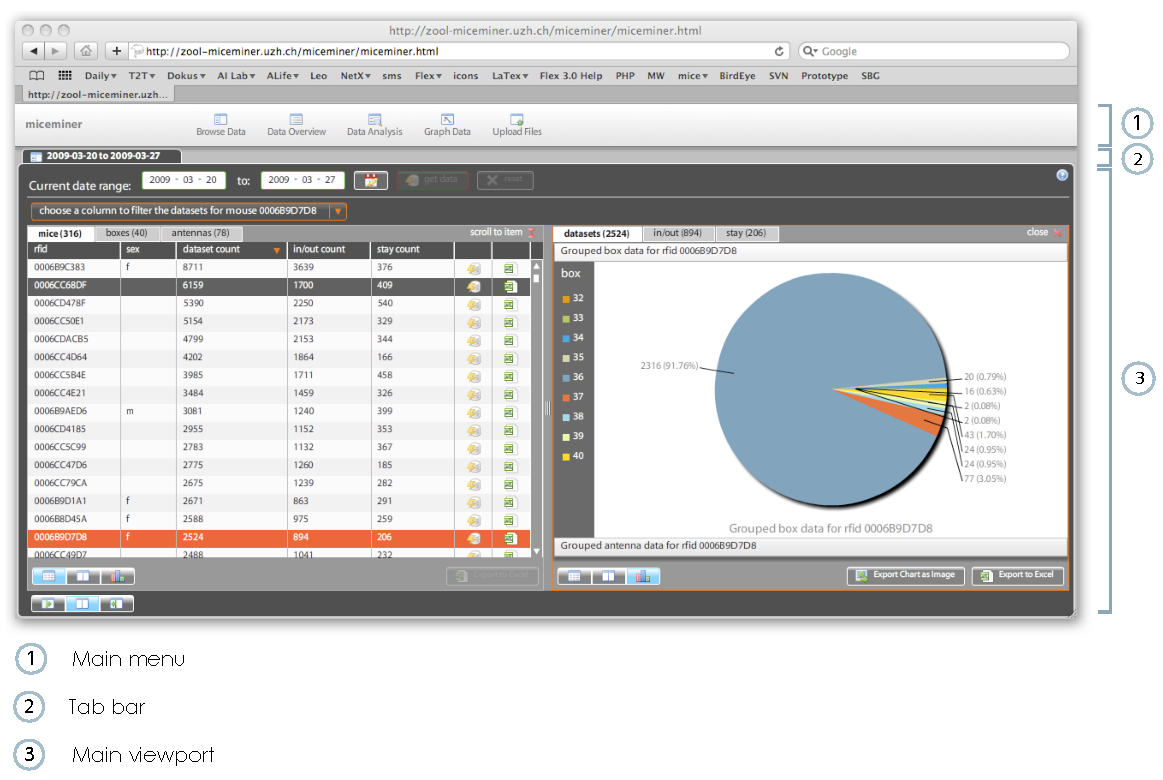
\includegraphics[width=\textwidth]{assets/pdf/interface_overview.pdf}
  \caption[miceminer interface overview]{Screenshot of the miceminer application displaying data for a mice.}
  \label{fig:interface_overview}
\end{center}
\end{figure}

From the \textit{main menu}, the user can choose from the following main components.

\subsubsection*{Browse Data}
This is the core component of the application and contains the functionality to explore the data in the database within a definable date range.

\subsubsection*{Data Overview}
Shows summarized information about all the mice, boxes antennas in the database.

\subsubsection*{Data Analysis}
Offers some simple data analysis and evaluation methods.

\subsubsection*{Graph Data}
Interactive network representation of a possible social network within the mice community.

\subsubsection*{Upload Files}
Components to perform administrative tasks. This component is password protected.

% \begin{figure}[htpb]
% \begin{center}
%   
\includegraphics[width=0.75\textwidth]{assets/img/main_menu.png}
%   \caption[miceminer main components]{The main components of the \textit{miceminer} application.}
%   \label{fig:main_components}
% \end{center}
% \end{figure}  


\subsection{Software design}
\label{subsec:miceminer_design}

\textit{Flex} itself does not include methods to query a database with \ac{SQL}. Instead the application sends it's request to a \textit{PHP}\footnote{PHP is a scripting language originally designed for producing dynamic web pages\cite{wiki:php}.} file stored on the server, containing the necessary methods. These methods handle the database queries and send the results back to the \textit{Flex} application, which is running on the client computer. An auxiliary software (\textit{AMFPHP}) speeds up the data transfer between the server and the client.

\textit{PHP} offers convincing ways to export the data to different file formats, including \textit{Excel} worksheets. \textit{Excel} export is available within most    

These interactions are illustrated in figure \ref{fig:app_design_miceminer}.

\begin{figure}[htpb]
\begin{center}
  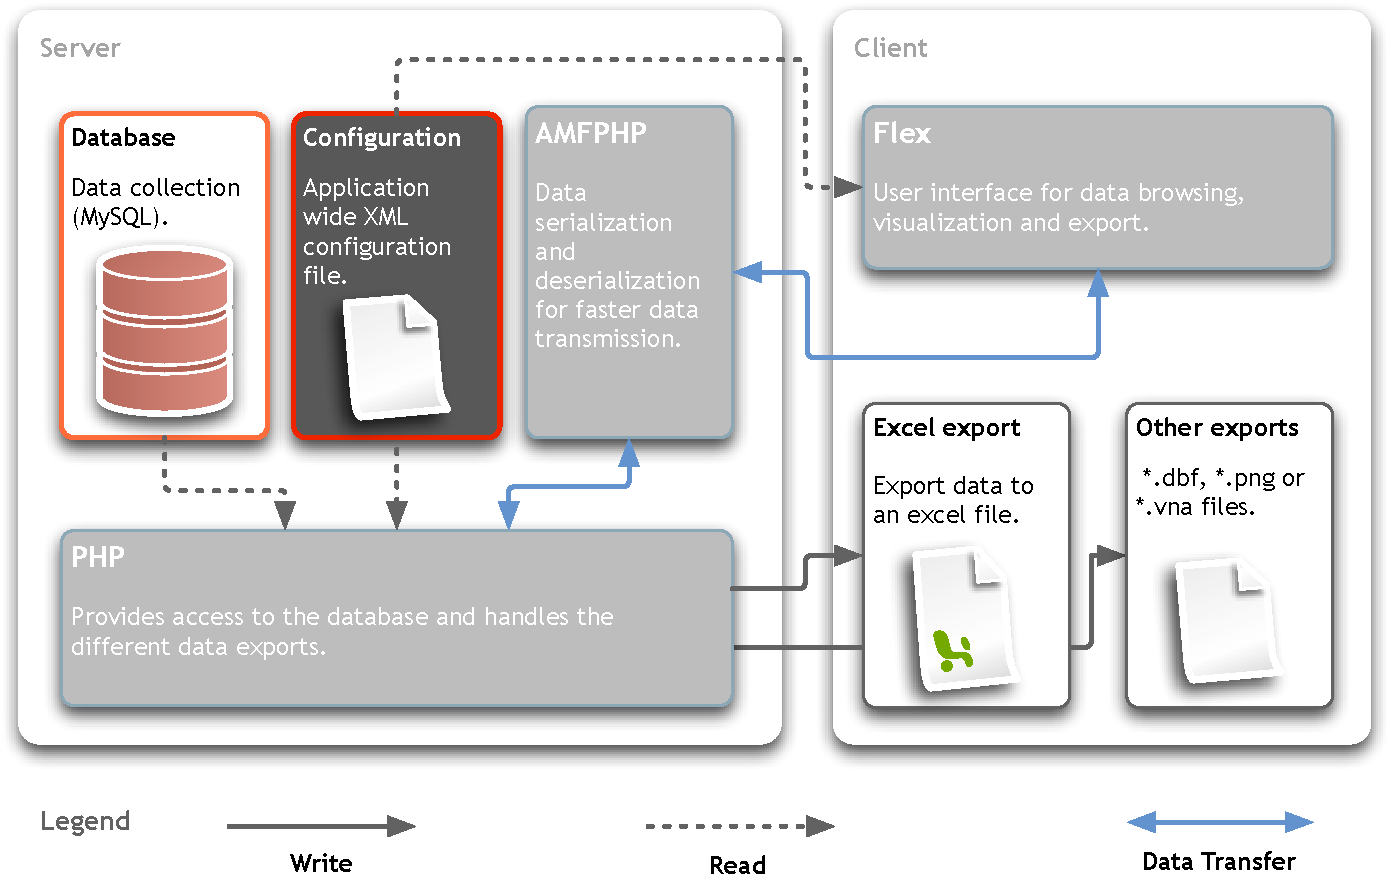
\includegraphics[width=\textwidth]{assets/pdf/application_design_miceminer.pdf}
  \caption[User Interface overview]{Overview of the parts involved in the user interface.}
  \label{fig:app_design_miceminer}
\end{center}
\end{figure}


\subsection{Configuration}
\label{subsec:miceminer_config}

\subsection{Data Filtering}
\label{subsec:datafilter}

Shortly explain the filtering possibilities of the program.

\subsection{Data Visualization}
\label{subsec:datavis}

Shortly explain the visualization possibilities of the program.

\subsection{Exporting Data}
\label{subsubsec:dataexp}

Shortly explain the export function of the program.

% ----------------------------------------------
% Data analysis
% ----------------------------------------------
\subsection{Simple data analysis with miceminer}
\label{subsec:dataana} 

Miceminer provides some simple data analysis functionality.

\subsubsection{Home Range Data}
\label{subsubsec:homerangedata} 

Functionality of the home range analysis.

Minimal polygon calculation for boxes area.
Applying threshold which boxes to take into account calculation. 

Exporting dbf files which can be imported into ARCGIS.

\paragraph{Applications}
Above method is outdated, nowadays Kernel Density Estimation is used -> Anna

\subsubsection{Shared Preferences}
\label{subsubsec:sharedpref} 

Is there a preference between to female mice.
Calculate if two females meet more often than expected, which lets us draw conclusions about a their relationship.

\paragraph{Applications}
Prof. Koenig ?

\subsubsection{Monthly Box}
\label{subsubsec:monthbox}

A matrix  showing which mice has been seen in which boxes over the selected time range.

\paragraph{Applications}
Prof. Koenig ?

\subsubsection{Monthly Antennas}
\label{subsubsec:monthant}

A matrix  showing which mice has been seen at which antennas over the selected time range.

\paragraph{Applications}
Prof. Koenig ?


% ===============================
% Network exploration
% ===============================
\section{Exploration of the social network data}
\label{sec:graph}

The visualization of somewhow pairwise connected data is ganining popularity in a broad variety of research fields. Mainly cause it as an attractive way to present the data, and facilitates the communication of complex interdependences within the data. Beyond the visualization, however, there is a variety of mathematical methods available to run statistical analysis over the data underlying the visualization. This makes the approach interesting as well for researchers using a more coventional statistical approach. Compared to the conventional approach, which is concerned with the monoadic attributes (e.g. sex, age, etc.) of the individuals, the \textit{Social Network Analysis} puts the dyadic attributes, the social relations between them, in the focus.

As well in biology, networks are widely used to visualize and analyse study, complex systems of correlated data. For example protein interactions, food webs or social behaviour of animals living in groups. However, especially for the latter one, little work has been done so far and only a handful of scientific papers have been published. The intersted reader is referred to the review entitled \textit{Social network analysis of animal behaviour: a promising 
tool for the study of sociality}\cite{wey:08} reviews and the excellent book \textit{Exploring Animal Social Networks}\cite{croft:07} containing an overview of the applications and possibilities to use the social network analysis in animal behaviour.

Since the data set collected for the conventional approach is perfect to get dyadic data\footnote{See the description of the meeting data in section \ref{subsec:meetingres} on page \pageref{subsec:meetingres}.}, and exceptionally large, it was clear that the \textit{miceminer} application should include tools which allow to use the data for social network analysis.

The next section contains a very short introduction to network theory, the theoretical fundament of the social network analysis. Thereafter, the concept and the actual implementation of the options in the \textit{miceminder} application are outlined.  

\subsection{Short introduction to network theory}
\label{subsec:graph_intro}

Please note that the following information are the basics of the network theory to understand the implementation of social network analysis tools in the \textit{miceminer} application. For an extensive introduction refer to the plenty of books, papers and online resources available.   

\subsubsection{Network types}
\label{subsubsec:net_types}
Depicted in figure \ref{fig:graph_undirected} is a very simple network with five nodes (A to D) and some (binary) edges between them. In social networks, the nodes, also called actors, are normally indviduals and the edges denote a relationship between them. For a train network, however, the nodes would stand for the train stations, and the edges for the connecting tracks.

Shown in figure \ref{fig:graph_undirected_weighted} is the same network as in figure \ref{fig:graph_undirected}, but with weighted edges. In addition to the binary edges, which just exist or not, the weighted edges illustrate the strenght of a connection. Reffering to the example with the train network, the weight or the thickness of the edge could stand for the traffic volume of the specific track. Or for a social network, the weight would indicate the strength of the social relation between the two individuals.  

\begin{figure}[htbp]
	\begin{minipage}[b]{0.5\textwidth}
    \captionsetup{width=.5\textwidth}
		\centering
			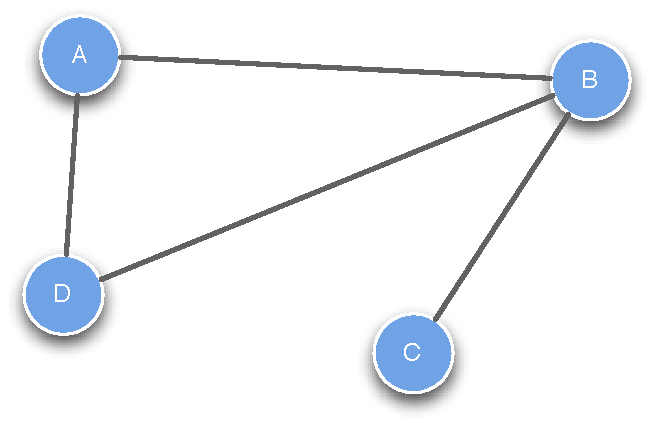
\includegraphics[width=0.5\textwidth]{assets/pdf/graph_undirected.pdf}
			\caption{Undirected network with binary edges.}
			\label{fig:graph_undirected}
	\end{minipage}
	\hspace{0.5cm}
	\begin{minipage}[b]{0.5\textwidth}
    \captionsetup{width=.5\textwidth}
		\centering
			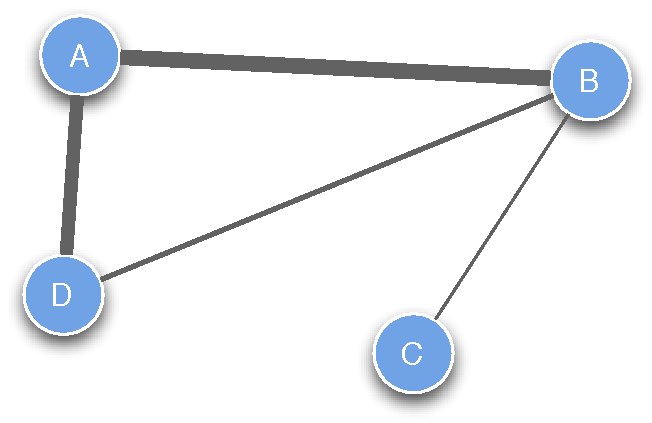
\includegraphics[width=0.5\textwidth]{assets/pdf/graph_undirected_weighted.pdf}
			\caption{Undirected network with weighted edges.}
			\label{fig:graph_undirected_weighted}
	\end{minipage}
\end{figure}

Another type of networks are the so called directed networks (see figures \ref{fig:graph_directed} and \ref{fig:graph_directed_weighted}). Unlike the undirected networks, the edges have a direction (usually depicted by an arrowhead). Applied to our real world model networks, the direction could represent a one way track of a train network, or the connection between a supplier and a customer. 

\begin{figure}[htbp]
	\begin{minipage}[b]{0.5\textwidth}
    	\captionsetup{width=.5\textwidth}
		\centering
			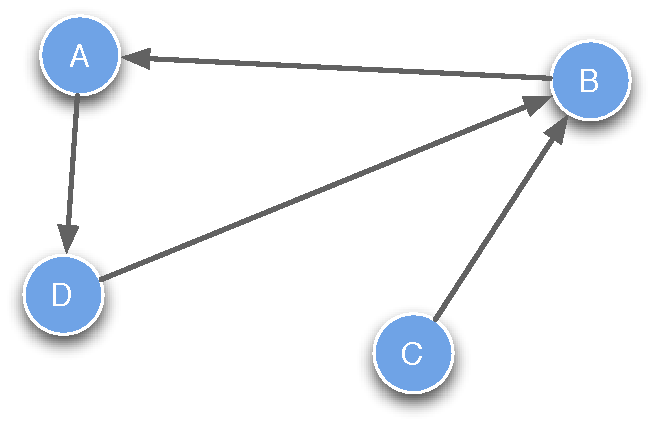
\includegraphics[width=0.5\textwidth]{assets/pdf/graph_directed.pdf}
			\caption{Directed network with binary edges.}
			\label{fig:graph_directed}
	\end{minipage}
	\hspace{0.5cm}
	\begin{minipage}[b]{0.5\textwidth}
    \captionsetup{width=.5\textwidth}
		\centering
			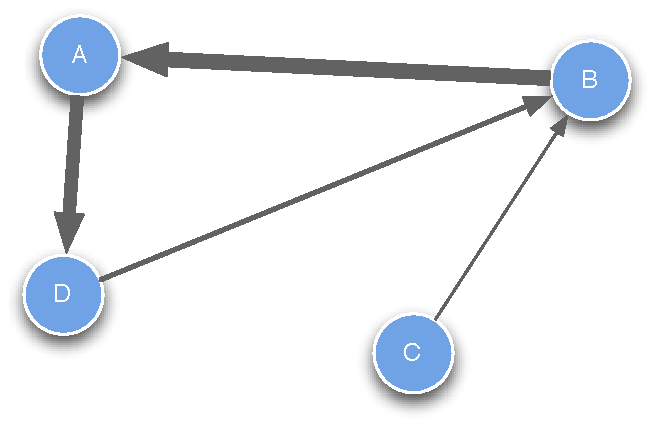
\includegraphics[width=0.5\textwidth]{assets/pdf/graph_directed_weighted.pdf}
			\caption{Directed network with weighted edges.}
			\label{fig:graph_directed_weighted}
	\end{minipage}
\end{figure}

There are plenty of other varieties of networks. But the ones described above are adequate to understand the visualization implemented in the \textit{miceminer} application.

\subsubsection{Adjacency matrix}
\label{subsubsec:adjacency_matrix}

The data underlying the visualization is a so called adjacency matrix. Table \ref{tab:am_undirected} shows the tabular reprsentation of the network shown in figure \ref{fig:graph_undirected} and the corresponding adjacency matrix alongside in figure \ref{fig:am_undirected}.

\begin{figure}[ht]
	\begin{minipage}[t]{0.5\textwidth}
    \captionsetup{width=.45\textwidth}
    \vspace{0pt}
		\centering
			\newcolumntype{H}{>{\bf}p{.5cm}}
			\begin{tabularx}{.5\textwidth}{+H|^X^X^X^X}
			\rowstyle{\bfseries}
				&	A	&	B	&	C	&	D \\\midrule
			A	&	0	&	1	&	0	&	1 \\
			B	&	1	&	0	&	1	&	1 \\
			C	&	0	&	1	&	0	&	0 \\
			D	&	1	&	1	&	0	&	0 \\	
			\end{tabularx}
			\captionof{table}{Tabular representation of the network shown in figure \ref{fig:graph_undirected}.}
			\label{tab:am_undirected}
	\end{minipage}
	\hspace{0.5cm}
	\begin{minipage}[t]{0.5\textwidth}
    \captionsetup{width=.5\textwidth}
    \vspace{0pt}
		\centering
		\[
		\begin{pmatrix}
        	0	&	1	&	0	&	1 \\
			1	&	0	&	1	&	1 \\
			0	&	1	&	0	&	0 \\
			1	&	1	&	0	&	0 \\
		\end{pmatrix} 
		\]
		\captionof{figure}{The adjacency matrix of the data shown in table \ref{tab:am_undirected}.}
		\label{fig:am_undirected}
	\end{minipage}
\end{figure}

For the model network with the weighted graph (figure \ref{fig:graph_undirected_weighted}) the tabular representation and the adjacency matrix looks like shown in table \ref{tab:am_undirected_weighted} and figure \ref{fig:am_undirected_weighted} (assuming that the maximum weight of an edge is 5).

An adjacency matrix for an undirected network is symmetrical by the diagonal, since the edges do not have any direction. 

\begin{figure}[ht]
	\begin{minipage}[t]{0.5\textwidth}
    \captionsetup{width=.45\textwidth}
    \vspace{0pt}
		\centering
			\newcolumntype{H}{>{\bf}p{.5cm}}
			\begin{tabularx}{.5\textwidth}{+H|^X^X^X^X}
			\rowstyle{\bfseries}
				&	A	&	B	&	C	&	D \\\midrule
			A	&	0	&	5	&	0	&	4 \\
			B	&	5	&	0	&	1	&	2 \\
			C	&	0	&	1	&	0	&	0 \\
			D	&	4	&	2	&	0	&	0 \\	
			\end{tabularx}
			\captionof{table}{Tabular representation of the network shown in figure \ref{fig:graph_undirected_weighted}.}
			\label{tab:am_undirected_weighted}
	\end{minipage}
	\hspace{0.5cm}
	\begin{minipage}[t]{0.5\textwidth}
    \captionsetup{width=.5\textwidth}
    \vspace{0pt}
		\centering
		\[
		\begin{pmatrix}
			0	&	5	&	0	&	4 \\
			5	&	0	&	1	&	2 \\
			0	&	1	&	0	&	0 \\
			4	&	2	&	0	&	0 \\	
		\end{pmatrix} 
		\]
		\captionof{figure}{The adjacency matrix of the data shown in table \ref{tab:am_undirected_weighted}.}
		\label{fig:am_undirected_weighted}
	\end{minipage}
\end{figure}

Consequently, for a directed network, as the one shown in figure \ref{fig:graph_directed}, the adjacency matrix does not show any symmetry (see table \ref{tab:am_directed} and figure \ref{fig:am_directed}).

\begin{figure}[ht]
	\begin{minipage}[t]{0.5\textwidth}
    \centering
    \captionsetup{width=.5\textwidth}
    \vspace{0pt}
			\newcolumntype{H}{>{\bf}p{.5cm}}
			\begin{tabularx}{.5\textwidth}{+H|^X^X^X^X}
			\rowstyle{\bfseries}
				&	A	&	B	&	C	&	D \\\midrule
			A	&	0	&	1	&	0	&	1 \\
			B	&	0	&	0	&	1	&	1 \\
			C	&	0	&	0	&	0	&	0 \\
			D	&	0	&	0	&	0	&	0 \\	
			\end{tabularx}
			\captionof{table}{Tabular representation of the network shown in figure \ref{fig:graph_directed}.}
			\label{tab:am_directed}
	\end{minipage}
	\hspace{0.5cm}
	\begin{minipage}[t]{0.5\textwidth}
    \captionsetup{width=.5\textwidth}
    \vspace{0pt}
		\centering
		\[
		\begin{pmatrix}
			0	&	1	&	0	&	1 \\
			0	&	0	&	1	&	1 \\
			0	&	0	&	0	&	0 \\
			0	&	0	&	0	&	0 \\	
		\end{pmatrix} 
		\]
		\captionof{figure}{The adjacency matrix of the data shown in table \ref{tab:am_directed}.}
		\label{fig:am_directed}
	\end{minipage}
\end{figure}

A special network is the so called \textit{Ego Network}. The ego network consists of a focal node, called the \textit{Ego}, and the nodes directly connected to \textit{Ego}, plus the edges between them. Illustrated in figure \ref{fig:graph_ego} is the ego network for node A within the undirected network shown in figure \ref{fig:graph_undirected}.

\begin{figure}[htpb]
\begin{center}
  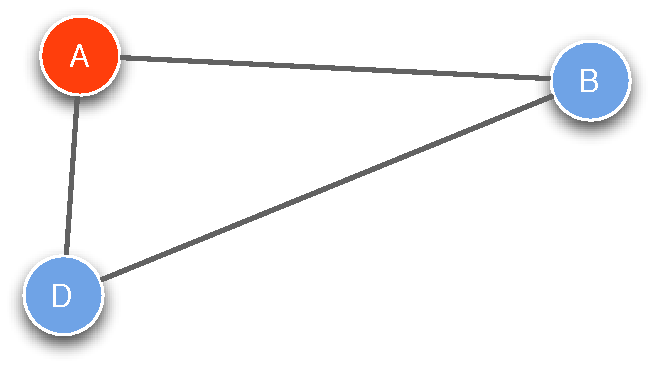
\includegraphics[width=.5\textwidth]{assets/pdf/graph_egocentric.pdf}
  \caption[Ego Network]{Ego Network for node A. The full network is shown in figure \ref{fig:graph_undirected} on page \pageref{fig:graph_undirected}.}
  \label{fig:graph_ego}
\end{center}
\end{figure} 

The adjacency matrix corresponding to a visualization, gives us the ability to characterize a network and make the actors comparable. These measurements are explained in the following sections.

\subsubsection{Network topology}
\label{subsubsec:topology}



\subsubsection{Node based measures}
\label{subsubsec:node_based}

In order to have some measures about a node in a network, values are defined to quantify the position of a node within a network. There are several of these so called node based measures available. Presented here are just the ones which are available in the \textit{miceminer} implementation.

The following methods to calculate the node based measures apply to networks with unweighted edges. Approaches are available, however, to calculate some of these measurements for networks with weighted edges. Though, the mathematics behind these methods is quite complex and most of the software available to analyse networks do not include possibilities to calculate these measures.

\paragraph{Average path length}

\paragraph{Clustering coefficient}

\paragraph{Degree}

\paragraph{Betweenness}

\subsection{Concept}
\label{subsec:graph_concept}

Social relations in the sense of this project are defined as the time two mice spend together in an artificial nestbox. This is an obvious approach. Mice only share an area at the same time voluntarily, if they have some kind of affirmative social relation.

Since the data includes information about the strength of the relationship, which is the actual time two mice spent together, the network has weighted edges. In some way, the data even includes directional information. As mentioned in the section about the meeting results, there are four different situations (meeting types) imaginable, how two mice can meet (see list \ref{list:meeting_types} and the corresponding figure \ref{fig:meeting_types}). Anyway, this information is not clearly unidirectional. Since the edges are made up of several different meetings, whereof never all of them are of the same meeting type, we do not have a directed graph.

Consequently, an undirected network with weighted edges is shown. The weight depends on the sum of time two mice spend together over a period of time. In addition, information about the composition (different meetings) of the edges is available.

The aim was not to build a comprehensive tool for social network analysis, as there are already plenty of them available. Instead, the component is intended to provide methods to carry out data mining of the network or meeting data. Similar to the component to browse the data, the user should be provided with a tidy interface presenting the main information and options: the visulization of the network and the corresponding node based values, as well as export options for further analysis in the preferred software.    

\subsection{Implementation}
\label{subsec:graph_explore}

Pictured in figure \ref{fig:graph_data_interface_overview} is an overview of the interface for the \textbf{Graph Data} component.

\begin{figure}[htpb]
\begin{center}
  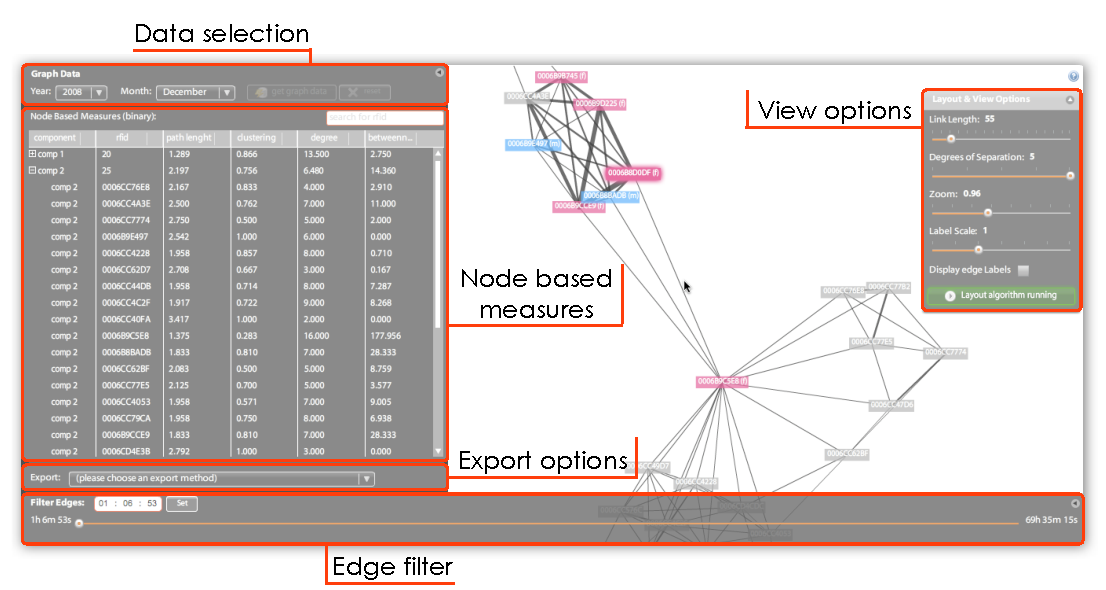
\includegraphics[width=\textwidth]{assets/pdf/graph_data_interface_overview.pdf}
  \caption[Graph Data interface overview]{Interface overview of the \textbf{Graph Data} component, including the identificaton of the main parts.}
  \label{fig:graph_data_interface_overview}
\end{center}
\end{figure}


\subsection{Possible research}
\label{subsec:graph_research}


% ===============================
% Conclusions
% ===============================
\newpage
\section{Conclusions}
\label{sec:concl}

... will see.

%---------------------------------------------------------------------------------------------------------
% Document References
%---------------------------------------------------------------------------------------------------------
\newpage
%\addcontentsline{toc}{section}{References}
\bibliographystyle{plainnat}
\bibliography{references}

% ===============================
% Appendix
% ===============================
\begin{appendix}
\addappheadtotoc
%---------------------------------------------------------------------------------------------------------
% Code
%---------------------------------------------------------------------------------------------------------
%---------------------------------------------------------------------------------------------------------
% Code
%---------------------------------------------------------------------------------------------------------
\newpage

% style for the perlscript code
\lstset{
	language=Perl,
	breaklines=true,
	showspaces=false,
	showstringspaces=false,
	showtabs=false,
	basicstyle=\scriptsize,
	numbers=left,
	numberstyle=\scriptsize,
	numbersep=3mm,
	stepnumber=1,
	backgroundcolor=\color{lightgrey},
	identifierstyle=\ttfamily,
	keywordstyle=\color[rgb]{0.08,0,0.81},
	commentstyle=\color[rgb]{0.33,0.33,0.33},
	stringstyle=\color[rgb]{1,0.12,0.58},
}

\section{Code}
\label{sec:code}

\subsection{Data processing scripts}
\label{subsec:dataprocscripts} 

\subsubsection{logimport.pl}
\label{code:logimport} 

\label{lst:antenna_adress_conversions}
\lstinputlisting[firstnumber=405,firstline=405, lastline=413, caption=Antenna address conversions]{/var/www/mouse/perl/import/logimport.pl}


\subsubsection{searchdir.pl}
\label{code:searchdir}

\lstinputlisting[firstnumber=0,firstline=0, lastline=10, label=lst:searchdir]{/var/www/mouse/perl/import/searchdir.pl}

\subsubsection{searchres.pl}
\label{code:searchres}

\lstinputlisting[firstnumber=0,firstline=0, lastline=10,label=lst:searchres]{/var/www/mouse/perl/import/searchres.pl}

%---------------------------------------------------------------------------------------------------------
% Code
%---------------------------------------------------------------------------------------------------------
\newpage
\section{Tables \& schemata}
\label{sec:tables_schmemata}

\begin{figure}[htpb]
\begin{center}
  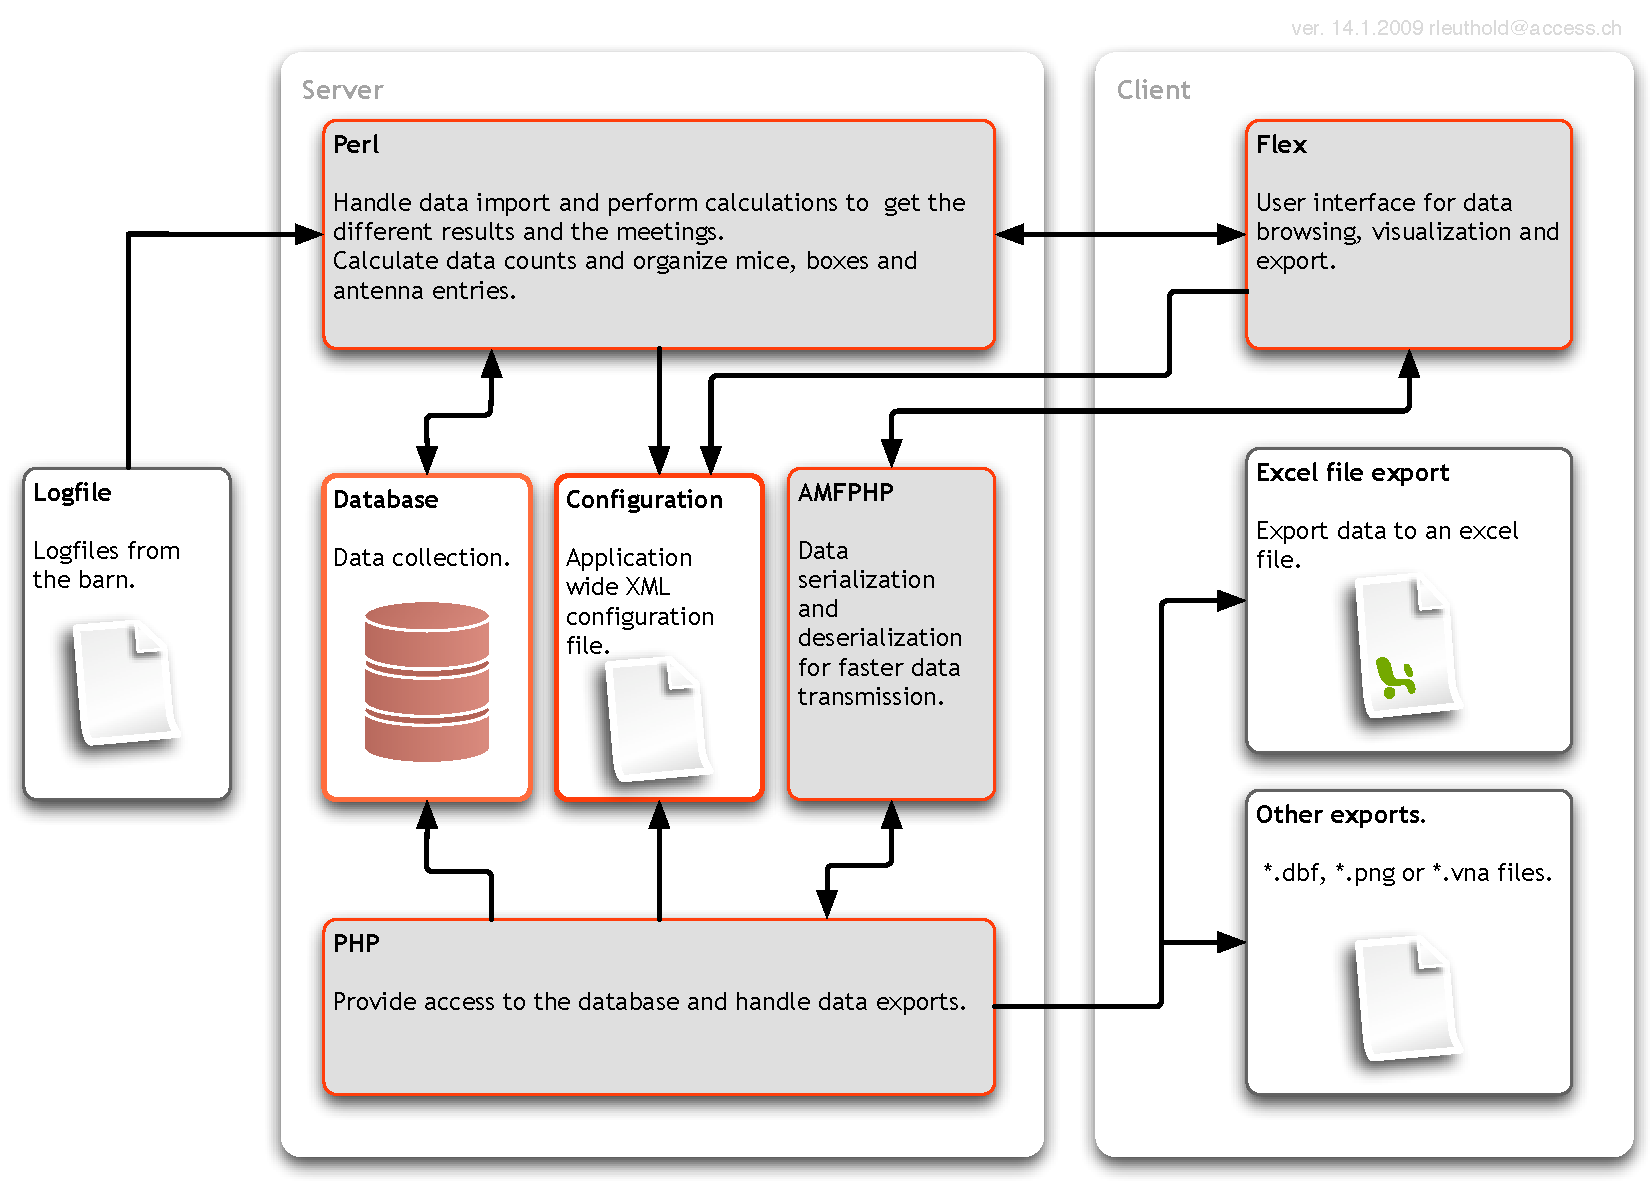
\includegraphics[width=\textwidth]{assets/pdf/app_design.pdf}
  \caption[Application design]{Overview of the application design.}
  \label{fig:app_design}
\end{center}
\end{figure}


% Micedata database schema
\begin{sidewaysfigure}
  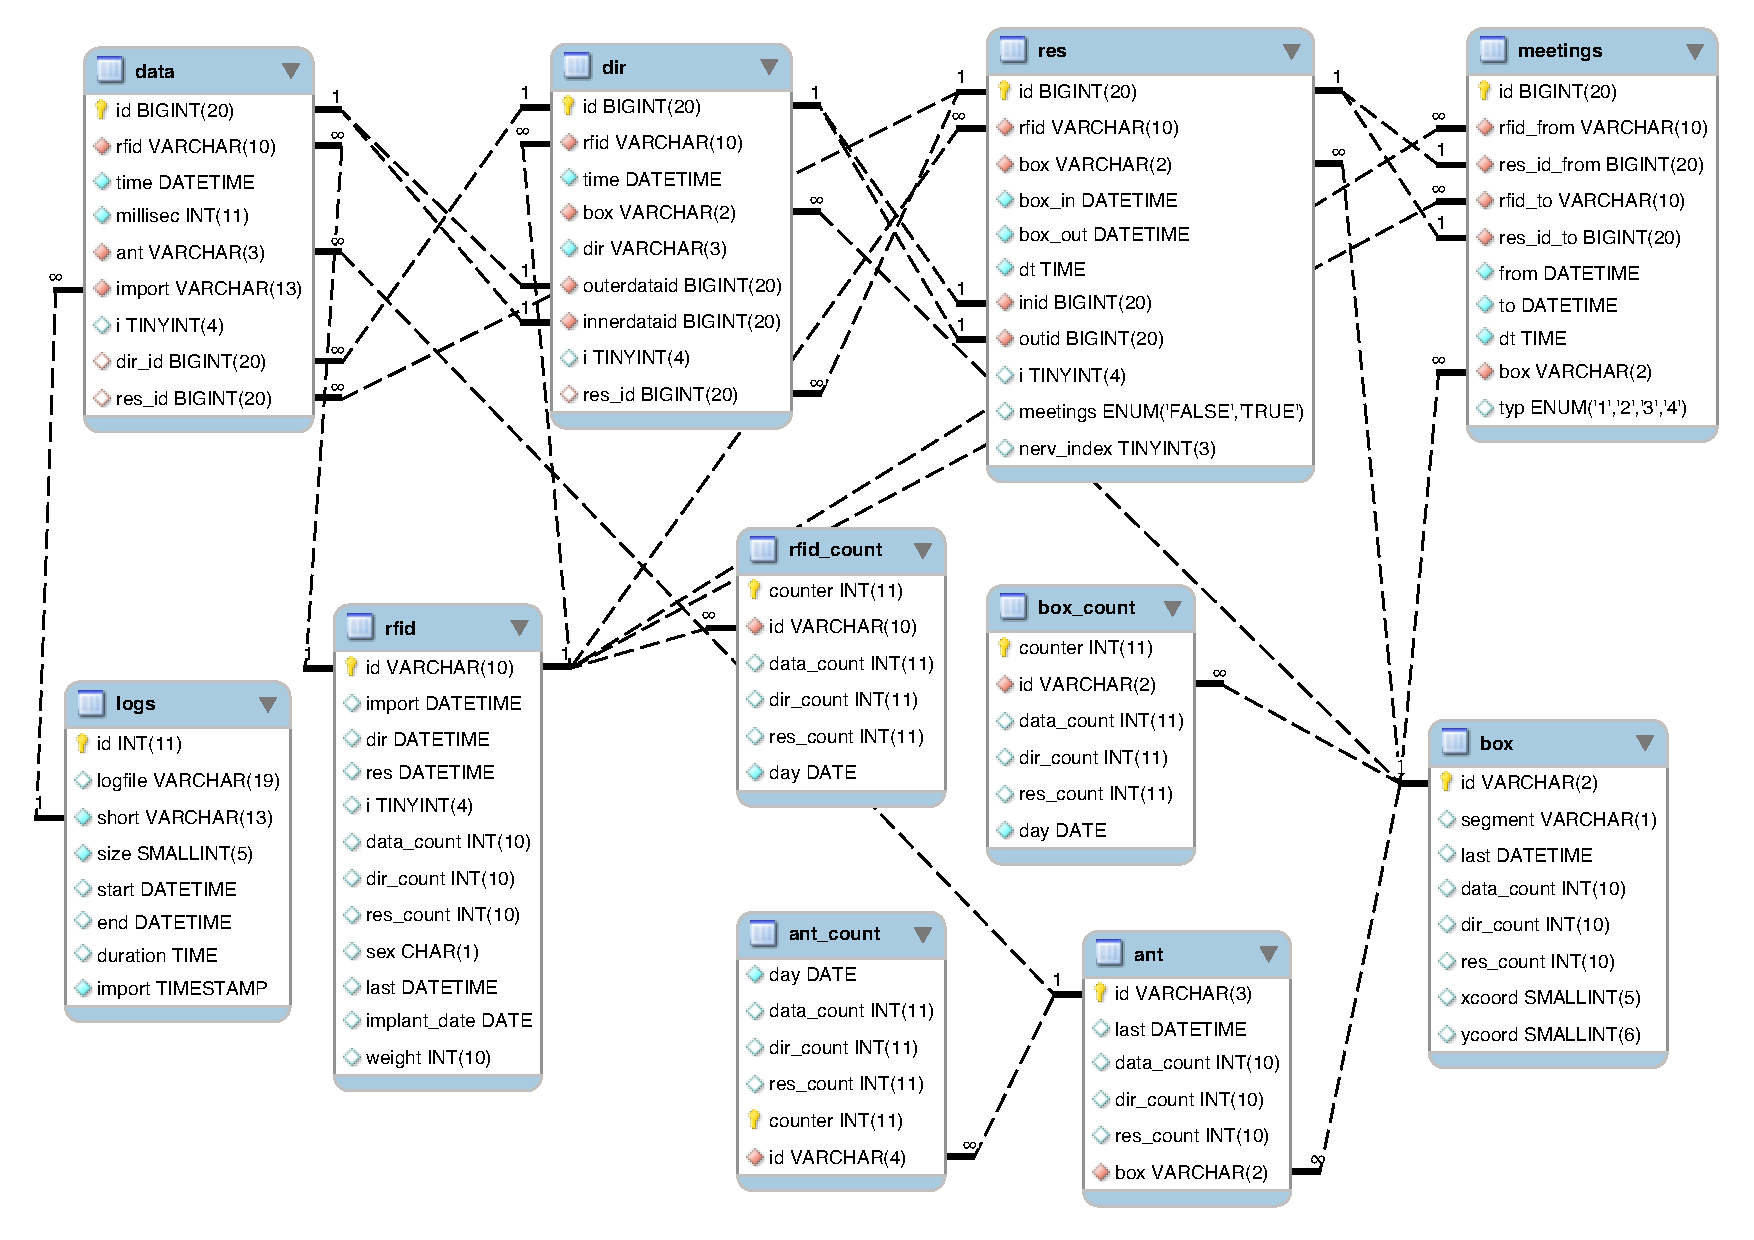
\includegraphics[width=\textwidth]{assets/pdf/micedata_schema.pdf}
  \caption[Database schema]{Database schema including all the tables and the relations between them.}
  \label{fig:database_schema}
\end{sidewaysfigure}

\begin{sidewaystable}
\newcolumntype{H}{>{\bf}lp{2.5cm}}
\caption{Meaning of the \lstinline|i| values in the database tables.}
\begin{tabularx}{\textheight}{+H^X^X^X^X^X}
\toprule
\rowstyle{\bfseries}
	&	\textbf{0}	&	1	&	2	&	3	&	4\\\midrule
data	    &  Dataset has not been analyzed yet.  &  Dataset has been analyzed but no matching dataset to form a \textit{direction result} could be found.	&	Dataset is part of a \textit{direction result} .	&	Dataset is part of a typ \textbf{3} \textit{stay result}.	&	Dataset is part of a typ \textbf{4} \textit{stay result}.\\\midrule

dir     	& \textit{Direction result} has not been analyzed yet. &  \textit{direction result} has been analyzed but no matching \textit{direction result} to form a \textit{stay result} could be found. & -  &  \textit{Direction result} is part of a typ \textbf{3} \textit{stay result}. & \textit{Direction result} is part of a typ \textbf{4} \textit{stay result}.\\\midrule

res     	& - & - & - & \textit{Stay result} is of typ \textbf{3} & \textit{Stay result} is of typ \textbf{4} \\\bottomrule
\label{tab:i_values}
\end{tabularx}

\end{sidewaystable}

% Micedata cheatsheet
\begin{sidewaysfigure}
  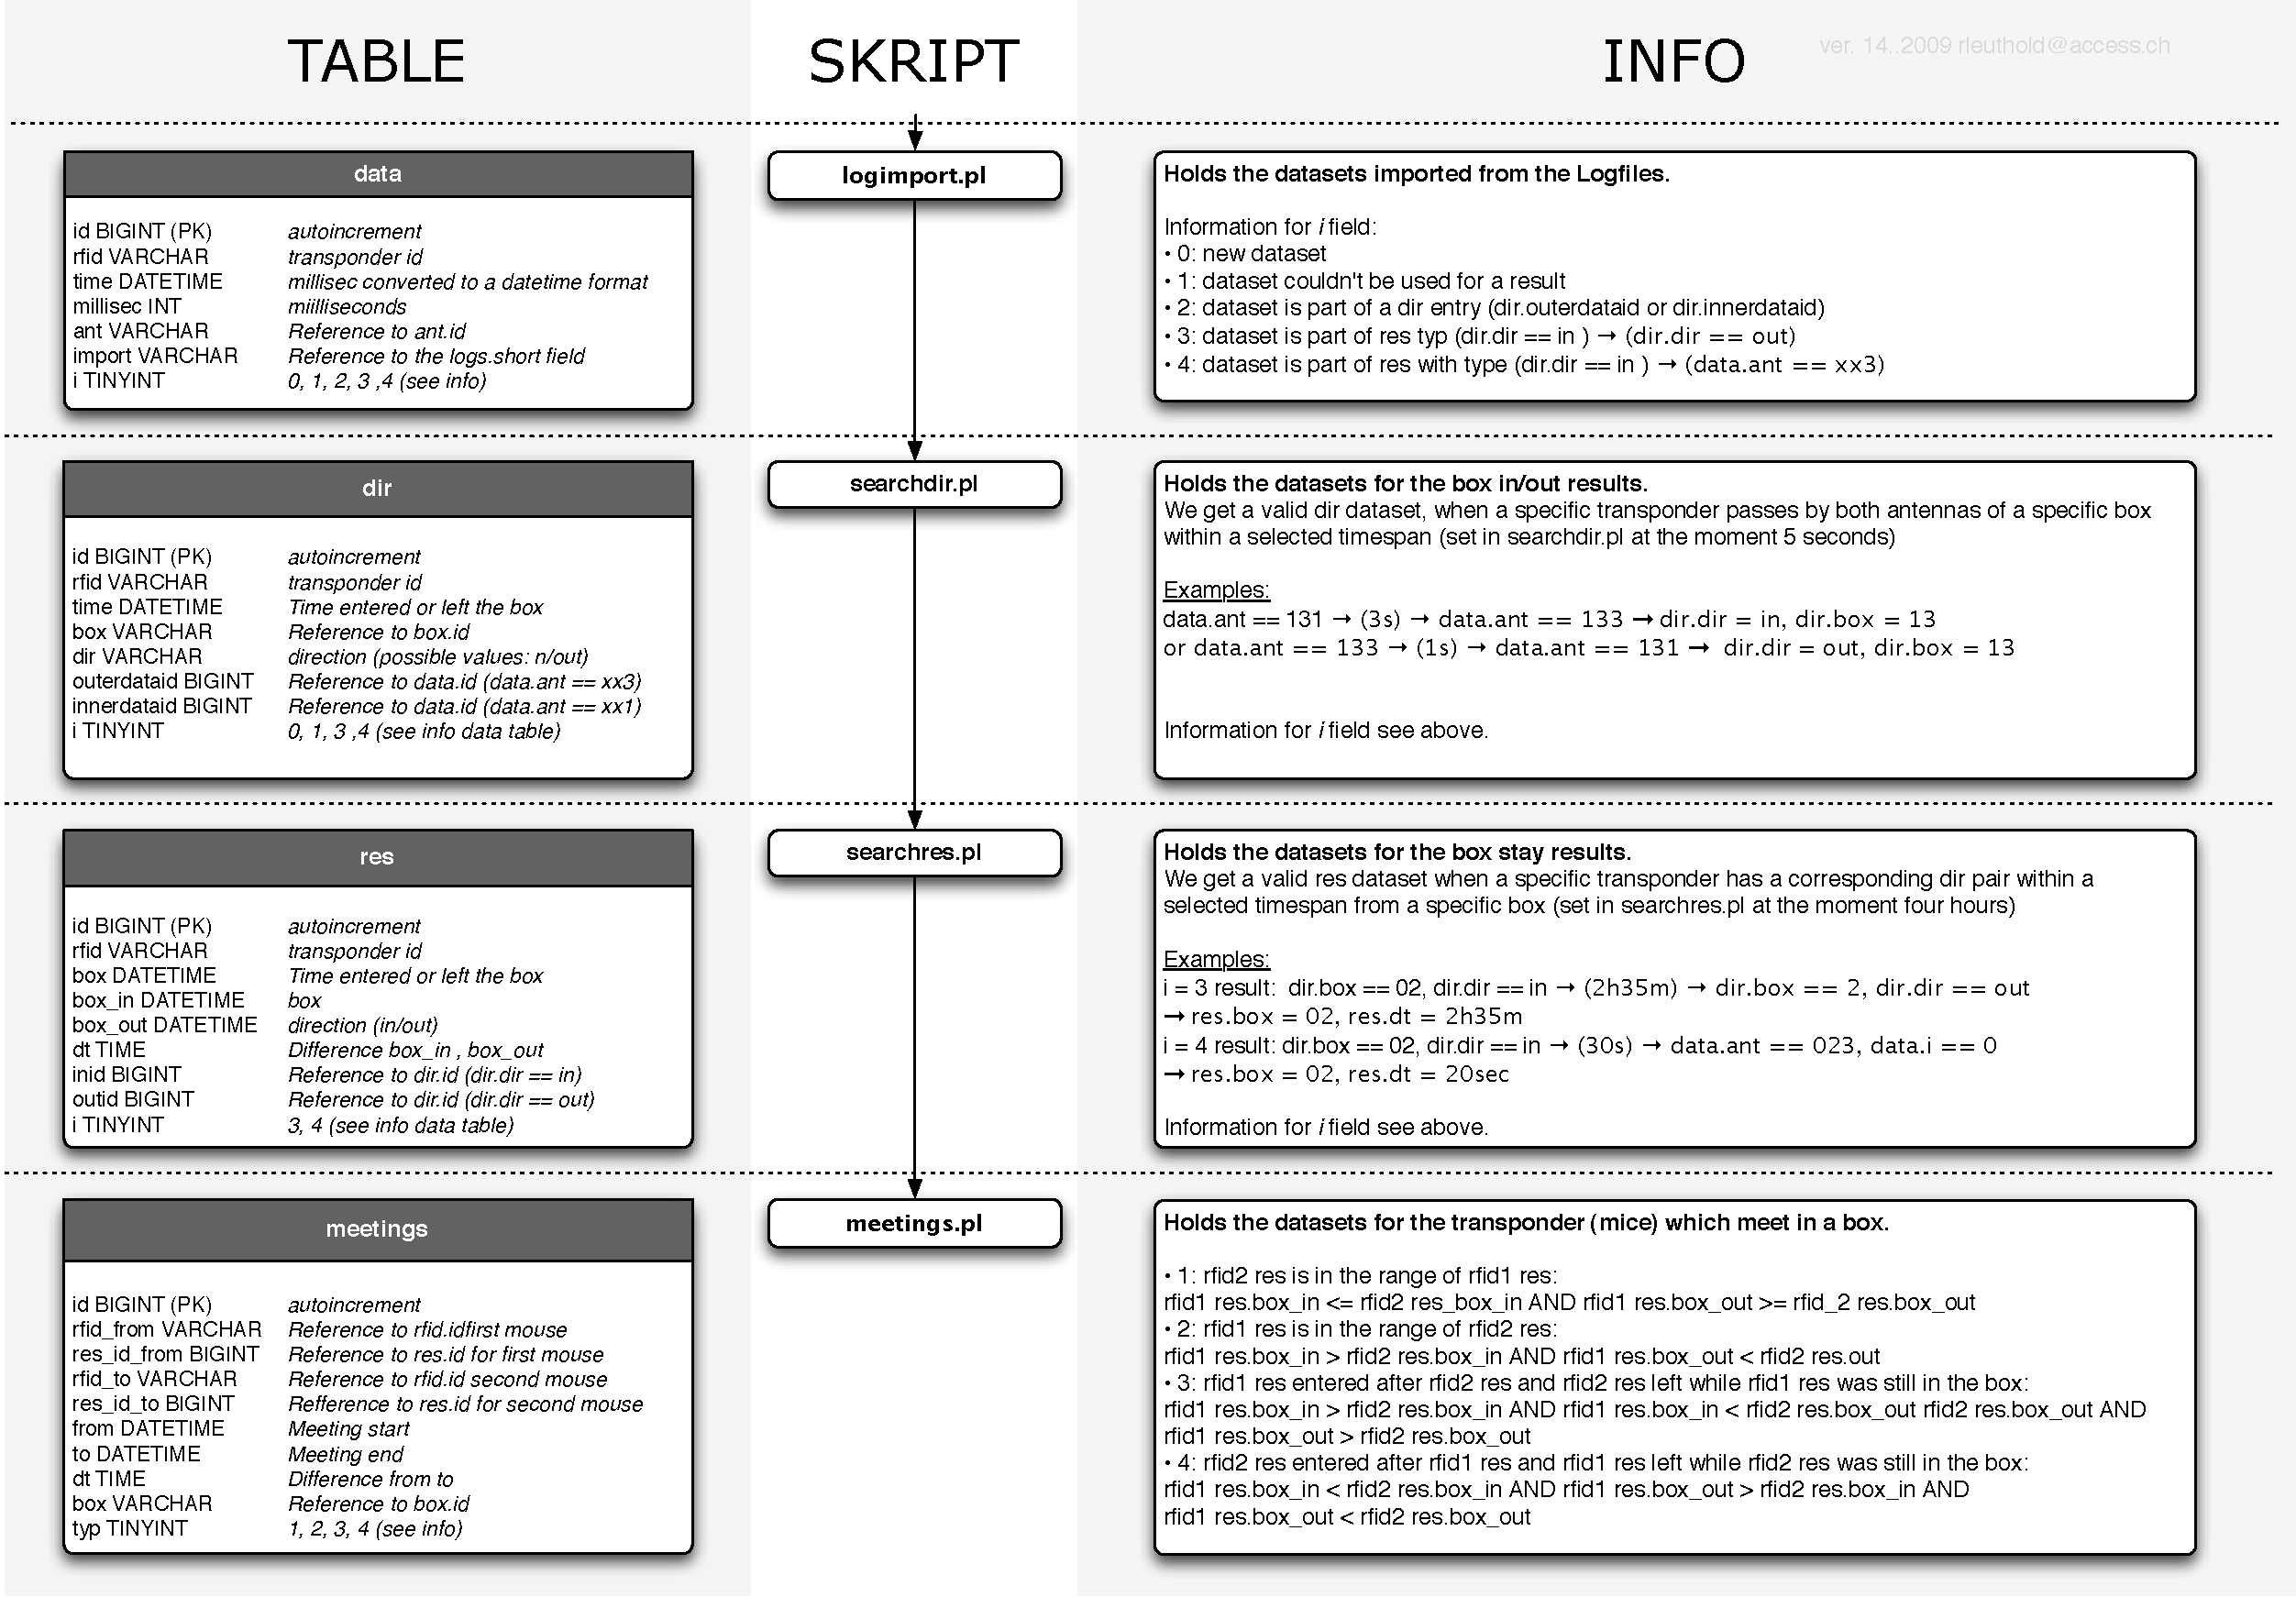
\includegraphics[width=\textwidth]{assets/pdf/micedata_data_processing_cheatsheet.pdf}
  \caption[Data processing cheatsheet]{Cheatsheet for the data processing steps.}
  \label{fig:data_processing_cheatsheet}
\end{sidewaysfigure}

\newpage

% Server information 
\subsection{Server information}
\label{subsec:server_information}

\subsubsection{General information}
\label{subsubsec:general_sys_info}
 
\begin{center} 
\newcolumntype{H}{>{\bf}p{2.5cm}}
\renewcommand\arraystretch{1.5}% (MyValue=1.0 is for standard spacing)
\begin{tabularx}{\textwidth}{+>{\raggedleft\arraybackslash}H^X}

\toprule
Model	& 	Dell Inspiron 530 \\\midrule
Processor	&	Intel(R) Core(TM)2 Duo CPU E7200  @ 2.53GHz, 2525 MHz \\\midrule
Memory (RAM)	&	2 GB \\\midrule
Operating system		&	Linux version 2.6.27-7-server  (gcc version 4.3.2 (Ubuntu 4.3.2-1ubuntu11) ) \\\midrule
IP-address	&	130.60.23.6 \\\midrule
Webserver	&	Apache/2.2.9 (Ubuntu) \\\midrule
SSH	&	OpenSSH 5.1p1  \\\midrule
PHP	version	&	5.2.6-2ubuntu4 \\\midrule
Perl version	&	 5.10.0 \\\bottomrule
\end{tabularx}
\captionof{table}{General information about the server}
\label{tab:server_information}
\end{center}

\newpage
% Web addresses
\subsubsection{Web addresses}
\label{subsubsec:urls}

\textbf{Please note that the server is only accessible from within the network of the \textit{University of Z\"urich}.}

\begin{center} 
\newcolumntype{H}{>{\bf}p{7cm}}
\renewcommand\arraystretch{1.2}% (MyValue=1.0 is for standard spacing)
\begin{tabularx}{\textwidth}{+>{\raggedright\arraybackslash}H^X}
\toprule
\rowstyle{\bfseries}
Address	&	Description \\\midrule
\url{http://zool-miceminer.uzh.ch}	&	Main Site containing containing a lot of information about the project. \\\midrule
\url{afp://zool-miceminer.uzh.ch}	&	\ac{AFP} access to the server. \\\midrule
\url{smb://zool-miceminer.uzh.ch}	&	\ac{Samba} access to the server. \\\midrule
\url{http://zool-miceminer.uzh.ch/phpmyadmin}	&	Web-based MySQL database administration tool (\href{http://www.phpmyadmin.net/}{phpMyAdmin}). \\\midrule
\url{http://zool-miceminer.uzh.ch/amfphp/browser/index.html}	&	\href{http://www.amfphp.org/}{AMFPHP} service browser. \\\midrule
\url{http://zool-miceminer.uzh.ch/webalizer}	&	Webserver traffic analyzer (\href{http://www.webalizer.org/}{Webalizer}). \\\midrule
\url{http://zool-miceminer.uzh.ch/miceminer/srcview/index.html}	&	Source of the \textit{miceminer} application. \\\midrule
\url{http://zool-miceminer.uzh.ch/asdoc/index.html}	& \textit{Adobe Flex} \ac{API} documentation of the \textit{miceminer} application. \\\midrule
\url{http://zool-miceminer.uzh.ch/conf/config.xml}	&	XML-based application wide configuration file (special login required). \\\midrule
\url{http://zool-miceminer.uzh.ch/conf/micedata_create.sql}	&	The SQL which are used to create the database structure (special login required). \\\bottomrule


\end{tabularx}
\captionof{table}{List of web addresses.}
\label{tab:web_addresses}
\end{center}

% Files and Directories
\subsubsection{Files \& directories overview}
\label{subsubsec:sys_directories}

\lstset{language=bash}
  

\begin{center} 
\newcolumntype{H}{>{\bf}p{5cm}}
\renewcommand\arraystretch{1.2}% (MyValue=1.0 is for standard spacing)
\begin{tabularx}{\textwidth}{+>{\raggedright\arraybackslash}H^X}
\toprule
\rowstyle{\bfseries}
Directory	&	Description \\\midrule
\lstinline|/var/www/mouse|	&	Base directory of the whole project relevant files and folders. \\\midrule
\\
\hline
\multicolumn{2}{|l|}{\textbf{All of the following files and directories are located within the base directory!}} \\
\hline
\\\midrule
\lstinline|conf/conf.xml|	&	The main \ac{XML} configuration file. \\\midrule
\lstinline|import_scripts//|	&	Contains the \ac{BASH} scripts to start the import cascade at a specific script (see \ref{app:import_schedule} on page \pageref{app:import_schedule} for details). \\\midrule
\lstinline|data/|	&	Uploaded but not yet imported data files. \\\midrule
\lstinline|data/cronlogs/|	&	Transcripts created the \ac{perl} scripts involved in the data import process. \\\midrule
\lstinline|data/imported/|	&	After successful import of a data file into the database, the file is moved into this directory.  \\\midrule
\lstinline|miceminer/|	&	The \textit{miceminer} application main files and folders.\\\midrule
\lstinline|perl/cgi|	&	\ac{CGI} scripts written in \ac{perl} which are used by the \textit{miceminer} application. \\\midrule
\lstinline|perl/extras/|	&	Perl scripts to control the data validity in the database and to compile data for some special analysis. The task of these scripts is usually explained in the header section of the file. \\\midrule
\lstinline|perl/import/|	&	Contains the perl script involved in the data import and processing. \\\midrule
\lstinline|perl/lib/|	&	The perl modules needed by all the import, reset and CGI scripts. \\\midrule
\lstinline|perl/reset/|	&	Scripts to set back the data in the database, so that the import scripts can be rerun. \\\midrule
\lstinline|amfphp/services/miceMiner/Mice.php|	&	\href{http://www.amfphp.org/}{AMFPHP} services file. \\\midrule
\lstinline|asdoc/|	&	Contains the \textit{miceminer} \ac{API} online documentation files. \\\bottomrule
\end{tabularx}
\captionof{table}{Overview of the important files and directories.}
\label{tab:directories_and_files_overview}
\end{center}

% import scripts
\newpage
\subsection{Starting \& scheduling import scripts}
\label{app:import_schedule}

To start the import cascade, a set of \ac{BASH} scripts is provided (see table \ref{tab:directories_and_files_overview} on page \pageref{tab:directories_and_files_overview} for the directoy these scripts are located in). Each of these scripts starts the import cascade at a specific per script and sends a mail including the transcript of the process to \href{mailto:miceminer@gmail.com}{miceminer@gmail.com} upon completion.

\begin{center} 
\newcolumntype{H}{>{\bf}p{5cm}}
\renewcommand\arraystretch{1.2}
\begin{tabularx}{\textwidth}{+>{\raggedright\arraybackslash}H^X}
\toprule
\rowstyle{\bfseries}
BASH script	&	perl script \\\midrule
\lstinline|import_step_1.sh|	&	\lstinline|logimport.pl| \\\midrule
\lstinline|direction_step_2.sh|	&	\lstinline|searchdir.pl| \\\midrule
\lstinline|results_step_3.sh|	&	\lstinline|searchres.pl| \\\midrule
\lstinline|meetings_step_4.sh|	&	\lstinline|meetings.pl| \\\midrule
\lstinline|counter_step_5.sh|	&	\lstinline|counter.pl| \\\midrule
\end{tabularx}
\captionof{table}{Overview of the BASH scripts and the perl import script they start.}
\label{tab:import_bash_scripts}
\end{center}
 
These scripts can be started manually from the command line or through a so called \textit{cronjob} which schedules the execution of the scripts.

\codefoot
\begin{lstlisting}[frame=none]
 # m h  dom mon dow   command
0 23 * * *      /var/www/mouse/import_scripts/import_step_1.sh   
\end{lstlisting}

The above listing shows the actual \textit{cronjob} which starts the import cascade every day at 11 o'clock p.m. beginning with the \lstinline|logimport.pl| script.

% configuration XML
\newpage
\subsection{Configuration}
\label{app:config} 

The application wide configuration is stored in a single XML file. The different possibilities to access or view the file can be found in the \ref{tab:directories_and_files_overview} table and the \ref{tab:web_addresses} table.

Please be careful on what you change. Never move the file to another location or delete it. Some minor knowledge in XML is advantageous to make changes in the configuration. It is strongly recommended to make a backup copy of the original file before applying changes. The file contains some explanations of what can be changed easely and what should not be changed.

\numcodestyle
\lstset{language=XML}    

\subsubsection{Database}
\label{app:configdb}

The following listing shows the part of the XML-configuration file responsible for the database connection to the \textit{MySQL} server. 

The values for the connection are set in the four nodes, \lstinline|<dbname>| contains the database name, \lstinline|<dbuser>| the user name, \lstinline|<dbpass>| the user password and \lstinline|<dbsocket>| the MySQL socket. This allows to switch the database, but only whne the table structures match (see the entry for the SQL file to create the database in table \ref{tab:web_addresses} on page \pageref{tab:web_addresses}).

The mapping to the database tables can be changed by setting the node value to another table, but only when the table structures match.

\subsubsection{Perl}
\label{app:configperl}

The perl part of the XML configuration file.

\lstinputlisting[firstnumber=59,firstline=59, lastline=70, caption=Perl configuration, label='lst:perl_config']{assets/code/config.xml}

\paragraph{scriptsFolder} The directory containing the perl \textit{Import Scripts} (see section \ref{sec:dataproc} on page \pageref{sec:dataproc} for details).

\paragraph{dbBackupUser} A MySQL user with \lstinline|SELECT| and \lstinline|LOCK TABLES| privileges on the database set as the \lstinline|<dbname>| value in the databse configuration (see appendix \ref{app:configdb} on page \pageref{app:configdb}). 

\paragraph{dbBackupDirectory} The directory in which the database backups are saved which are created at the beinning of the data import process.

\paragraph{antennaInterval}
\label{para:perl_antenna_interval}
Number of seconds that are allowed to elapse between the transponder readings at the inner and the outer antenna of box, to form a valid \textit{direction result}. 

\subsubsection{GUI \& PHP}
\label{app:configfrontend}
\lstinputlisting[firstnumber=82,firstline=82, lastline=83, caption=Maximum hours of stay results, label=lst:stay_config]{assets/code/config.xml}

\lstinputlisting[firstnumber=84,firstline=84, lastline=111, caption=Components configuration, label=lst:comp_config]{assets/code/config.xml}

Shown in the next listing is the beginning of the configuration for the grids in the GUI. The different part of the configuration is explained on the spot in the configuration file.

\lstinputlisting[firstnumber=418,firstline=418, lastline=468, caption=sample Grid configuration, label=lst:grid_config]{assets/code/config.xml}

%---------------------------------------------------------------------------------------------------------
% Glossary
%---------------------------------------------------------------------------------------------------------
\newpage

\section{Glossary}
\begin{acronym}
\acro{RDBMS}[Relational Database Management System]{A Relational Database Management System is a \acs{DBMS} in which data is stored in the form of tables and the relationship among the data is also stored in the form of tables \cite{wiki:rdbms}.}
\acro{DBMS}[Database Management System]{A Database Management System is computer software that manages databases \cite{wiki:dbms}.}
\acro{RFID}[Radio-frequency identification]{Radio-frequency identification (RFID) is the use of an object (typically referred to as an RFID tag) applied to or incorporated into a product, animal, or person for the purpose of identification and tracking using radio waves \cite{wiki:rfid} }
\acro{SQL}[Structured Query Language]{The Structured Query Language is a database computer language designed for the retrieval and management of data in relational database management systems.\cite{wiki:sql}}
\acro{KJ}[KJ]{The Joule is a derived unit of energy and defined as the work done by a force of one newton travelling through a distance of one metre. \cite{wiki:joule}. 1 Kilo Joule = 10$^3$ Joule.}
\acro{perl}[perl]{Perl is a high-level, general-purpose, interpreted, dynamic programming language. \cite{wiki:perl}}
\acro{PVC}[PVC]{Polyvinyl chloride is a widely used thermoplastic polymer \cite{wiki:pvc}}
\acro{GUI}[GUI]{A graphical user interface is a type of user interface which allows people to interact with electronic devices such as computers [\ldots] with images rather than text commands \cite{wiki:gui}}
\acro{API}[API]{An application programming interface is a set of routines, data structures, object classes and/or protocols provided by libraries and/or operating system services in order to support the building of applications \cite{wiki:api}.}
\acro{AFP}[AFP]{The Apple Filing Protocol is a network protocol that offers file services for Mac OS X \cite{wiki:afp}.}
\acro{Samba}[Samba]{Samba allows file and print sharing between computers running Windows and computers running Unix \cite{wiki:samba}.}
\acro{XML}[XML]{Extensible Markup Language is a general-purpose specification for creating custom markup languages \cite{wiki:xml}.}
\acro{CGI}[CGI]{The Common Gateway Interface is a standard protocol for interfacing external application software with an information server, commonly a web server \cite{wiki:cgi}.}
\acro{BASH}[BASH]{Bourne-again shell is a free software Unix shell written for the GNU Project /cite{wiki:bash}.}
\end{acronym}

\end{appendix}
%---------------------------------------------------------------------------------------------------------
% End Document
%---------------------------------------------------------------------------------------------------------
\end{document}